% The Bottleneck Effect: When Small-Model Scaling Fails for Code Generation
% Elsevier / SCP transfer build

\documentclass[preprint,12pt,authoryear]{elsarticle}
\usepackage[utf8]{inputenc}
\usepackage{amsmath}
\usepackage{amssymb}
\usepackage{graphicx}
\graphicspath{{outputs/figures/}}
\usepackage{url}
\usepackage{booktabs}
\usepackage{tabularx}
\usepackage{float}
\usepackage[protrusion=true,expansion=false]{microtype}
\usepackage[hidelinks]{hyperref}
\newcommand{\submissionartifact}{curated supplementary artifact archive}
\emergencystretch=4em

\journal{Science of Computer Programming}

\begin{document}

\begin{frontmatter}

\title{The Bottleneck Effect: When Small-Model Scaling Fails for Code Generation}

\author[inst1]{Ashish Pandey}
\ead{ashishpanday9818@gmail.com}

\affiliation[inst1]{
  organization={Department of Computer and Electronics Engineering, Khwopa College of Engineering},
  country={Nepal}
}

\begin{abstract}
Code generation is an execution-constrained software-engineering task: generated programs must parse, run, and satisfy tests. This paper studies whether small-model code generation improves with parameter scaling, code-specialized pretraining, and more distributed layerwise computation. Across HumanEval, MBPP, EvalPlus HumanEval+/MBPP+, and LiveCodeBench release v2, GPT-2 Medium (355M) does not reliably improve over GPT-2 Small (124M): the HumanEval gap is not statistically significant, and both GPT-2 variants reach 0.0\% success on full-coverage MBPP. In contrast, similarly sized CodeGen checkpoints retain substantially stronger executable-code behavior on HumanEval and MBPP. A fixed-scale CodeGen-350M NL$\rightarrow$Multi$\rightarrow$Mono ladder further shows that later code- and Python-focused continued pretraining improves the strongest checkpoint, especially on MBPP. To examine where these differences arise, we combine full-layer ablation, graded ablation, failure-mode analysis, and sparse activation steering. GPT-2 Medium is globally brittle under layer removal, while CodeGen retains residual success across several layers. A compact GPT-2 Medium layer-12 probe captures most of the success-vs.-syntax signal, but matched controls make the steering result suggestive rather than definitive. Overall, the results support a software-engineering reliability view: in this small-model regime, useful code behavior depends less on parameter count alone than on code-specific pretraining, generation protocol, and the distribution of execution-relevant computation across depth.
\end{abstract}

\begin{keyword}
code generation \sep empirical software engineering \sep large language models \sep model evaluation \sep mechanistic interpretability \sep software reliability
\end{keyword}

\end{frontmatter}

\section{Introduction}

Neural language-model scaling reliably improves average loss~\cite{kaplan2020scaling,hoffmann2022training}, and larger code models can improve program-synthesis benchmarks~\cite{austin2021program}. But code generation is not only a next-token prediction problem: a completion must parse, execute, and satisfy tests. It is therefore not obvious that modest parameter scaling within a general-language model family should improve execution reliability once code-specific pretraining and layerwise organization differ.

We study that gap in the small-model regime. On the HumanEval Python programming benchmark~\cite{chen2021humaneval}, GPT-2 Medium (355M parameters) reaches \textbf{4.8\% success}, statistically indistinguishable from GPT-2 Small (124M parameters) at \textbf{5.2\% success}. Yet CodeGen-350M~\cite{nijkamp2022codegen}---with nearly identical parameter count to GPT-2 Medium---reaches \textbf{37.4\% success}, a 7.8$\times$ improvement. The same ordering persists on the full MBPP test split: both GPT-2 models fall to \textbf{0.0\% success}, while CodeGen still reaches \textbf{7.39\% success}. Under stricter EvalPlus re-scores, both GPT-2 variants remain at \textbf{0.0\% pass@1} on HumanEval+ and \textbf{0.0\% on pass@1 and pass@10} on MBPP+, while CodeGen retains \textbf{2.1\% pass@1} on HumanEval+ and \textbf{1.1\% / 6.4\%} on MBPP+. A contamination-aware LiveCodeBench stress test is harsher for all three small models: GPT-2 Small and GPT-2 Medium both remain at \textbf{0.0\%} on pass@1, pass@5, and pass@10, while CodeGen is only marginally nonzero at \textbf{0.02\%, 0.10\%, and 0.20\%}. Finally, a within-family CodeGen-350M continued-pretraining ladder (NL$\rightarrow$Multi$\rightarrow$Mono) shows that Mono is best on both HumanEval and MBPP, with MBPP becoming cleanly monotone and HumanEval remaining mixed at the intermediate Multi checkpoint. These results motivate a narrower question than whether scale helps in general: \emph{when models are similarly small, what architectural properties let some of them organize executable-code behavior more effectively than larger general-language baselines?}

\subsection{The Bottleneck Hypothesis}

We hypothesize that code generation performance depends not on parameter count but on how models distribute code-relevant computation across layers. Specifically, we propose that models with brittle, sharply concentrated layerwise processing collapse under harsh interventions, while models with more distributed processing retain partial residual performance and more diverse failure signatures.

To test this hypothesis, we conduct systematic layer-wise ablation experiments: for each layer in each model, we zero out all activations and measure the impact on code generation success. This intervention reveals which layers are especially damaging when removed and how the resulting failure modes differ across architectures.

\subsection{Research Questions and Evidence Map}

We organize the study around four research questions. This framing is useful because code generation quality is not a single scalar property: the same model can differ in benchmark success, strict-test robustness, failure mode, and intervention sensitivity.

\begin{table}[H]
\centering
\caption{Research Questions, Evidence, and Main Takeaways}
\label{tab:rq_map}
\scriptsize
\begin{tabularx}{\columnwidth}{@{}>{\raggedright\arraybackslash}p{0.23\columnwidth}>{\raggedright\arraybackslash}X>{\raggedright\arraybackslash}p{0.30\columnwidth}@{}}
\toprule
\textbf{Question} & \textbf{Evidence Used} & \textbf{Takeaway} \\
\midrule
RQ1: Does GPT-2 scaling help? & HumanEval, MBPP, EvalPlus, LiveCodeBench & No reliable GPT-2 Small$\rightarrow$Medium gain. \\
RQ2: Does code pretraining matter? & GPT-2 vs. CodeGen; CodeGen ladder & Yes; code-specialized checkpoints are stronger. \\
RQ3: What changes under intervention? & Full/graded ablation and failure modes & GPT-2 Medium is brittle; CodeGen is more distributed. \\
RQ4: Is there a compact control signal? & Layer-12 probe and matched-control steering & Locally useful, but not yet definitive. \\
\bottomrule
\end{tabularx}
\end{table}

\subsection{Key Findings}

Through ablation of all 56 layers across three models (GPT-2 Small: 12 layers, Medium: 24 layers, CodeGen: 20 layers) evaluated on 16{,}300--16{,}400 code generation attempts, we find:

\begin{enumerate}
\item \textbf{The GPT-2 scaling gap is numerically small on HumanEval and disappears on MBPP}: GPT-2 Small exceeds GPT-2 Medium by only 0.37 percentage points on HumanEval (95\% CI $[-0.73, 1.37]$, $p=0.50$), while both score 0.0\% on full-coverage MBPP.

\item \textbf{GPT-2 Medium is globally fragile but has a distinctive mid-depth failure mode}: every GPT-2 Medium layer ablation reduces success to 0\%, but ablating layer 12 uniquely converts 23.9\% of failures from syntax errors into runtime errors, indicating a special role in producing executable-but-incorrect code.

\item \textbf{CodeGen exhibits broader residual robustness}: under the same harsh intervention, CodeGen retains nonzero success in four layers (5, 7, 13, 18), with layer 13 preserving 29.5\% success rather than collapsing completely. Under graded attenuation, the same layer still retains 28-30\% success at scales 0.75 and 0.5.

\item \textbf{A graded pilot sharpens the layer-12 interpretation}: on a 10-problem / 5-sample subset, scaling layer 12 from 1.0 to 0.5 and 0.25 first pushes GPT-2 Medium toward near-total syntax collapse, while only full zeroing reproduces the runtime-error regime (28.0\%), indicating a thresholded execution checkpoint.

\item \textbf{A compact probe captures most of the layer-12 linear signal}: five dimensions (121, 346, 615, 820, 169) in GPT-2 Medium's layer 12 achieve 72.5\% held-out success-vs.-syntax classification accuracy, compared with 75.0\% for the full 1024-dimensional layer.

\item \textbf{Constructive steering is useful but only suggestively specific}: steering GPT-2 Medium along the learned top-5 layer-12 vector raises subset success from 6.0\% to 12.0\% at $\alpha=2.0$. Against 20 matched sparse random controls, the learned vector beats 19 and exceeds the control mean (6.2\%), but one control reaches 14.0\%, so the specificity evidence is promising rather than definitive.

\item \textbf{The scaling failure transfers across benchmarks and stricter tests}: on full-coverage MBPP (257 tasks, 20 samples each), both GPT-2 variants remain at 0.0\% success, whereas CodeGen reaches 7.39\% success and 22.96\% pass@5 with highly significant pairwise gaps ($p=0.0001$). Under a stricter HumanEval+ re-score on the first five saved samples per task, both GPT-2 variants stay at 0.0\% pass@1 while CodeGen retains 2.1\%. On contamination-aware LiveCodeBench release v2~\cite{jain2024livecodebench}, both GPT-2 variants remain at 0.0\% on pass@1, pass@5, and pass@10 and CodeGen remains only marginally nonzero, showing that all three small models are near-zero on a substantially harder modern benchmark.

\item \textbf{A within-family CodeGen ladder strengthens the pretraining argument}: in the 350M CodeGen NL$\rightarrow$Multi$\rightarrow$Mono continued-pretraining ladder, Mono is strongest on both benchmarks. On full-coverage HumanEval it reaches 39.0\% success, significantly above both NL (31.60\%) and Multi (30.66\%), while NL vs.\ Multi is not significant. On MBPP the ladder is cleanly monotone (0.02\%$\rightarrow$1.23\%$\rightarrow$2.76\%), with significant NL$<$Multi and Multi$<$Mono improvements. We therefore interpret the ladder as evidence about continued-pretraining plus curriculum effects rather than a perfectly factorized distribution-only ablation.

\item \textbf{Prompt and decoding controls expose systems-level bottlenecks}: targeted robustness controls show that prompt format and decoding temperature can change success substantially without changing model size. On HumanEval, CodeGen-Mono moves from 42.6\% success under signature-only prompts to 71.2\% under comment-plus-signature prompts. On MBPP, low temperature increases successful samples for both CodeGen-Mono and Qwen2.5-Coder, but reduces distinct-task coverage relative to standard decoding.

\item \textbf{Error profiles differ across checkpoints}: GPT-2 models produce 28.7\% indentation errors and 8.1\% keyword errors, while CodeGen produces 23.1\% bracket errors and 7.4\% indentation errors, revealing a distinct syntax-error profile without isolating the source of that difference.
\end{enumerate}

\subsection{Contributions}

This work makes four primary contributions:

\begin{enumerate}
\item \textbf{Empirical}: We document a negative small-model scaling result in code generation through evaluation on HumanEval, strict HumanEval+ and MBPP+ re-scoring with EvalPlus~\cite{liu2023evalplus}, full-coverage MBPP, and a contamination-aware LiveCodeBench stress test across three model scales.

\item \textbf{Methodological}: We combine sample-level evaluation with problem-level bootstrap confidence intervals, paired permutation tests, hard layer ablation, graded ablation, and matched-control activation steering to study code-generation failures from both statistical and mechanistic angles.

\item \textbf{Mechanistic}: We identify a compact layer-12 activation subspace that captures most of the linear probe performance, show that graded weakening of layer 12 reproduces the same execution-relevant transition seen under full ablation, and show that constructive steering along this subspace improves execution while yielding suggestive, but not yet definitive, evidence of specificity over matched sparse random controls.

\item \textbf{Software-engineering reliability}: We show that reported code-generation reliability depends on more than checkpoint size: code-specific pretraining, the distribution of executable-code behavior across depth, prompt format, decoding policy, and task-level coverage all affect whether generated programs actually run and pass tests. A within-family CodeGen continued-pretraining ladder further shows that architecture-matched checkpoints can still diverge substantially as code- and Python-specific pretraining accumulates.
\end{enumerate}

These findings challenge the assumption that parameter scaling alone improves code generation, suggesting that in this small-model regime pretraining specialization and the distribution of execution-relevant computation across layers are more informative than model size alone.

\section{Related Work}

\subsection{Code Generation Models}

Recent progress in neural code generation follows from scaling language models trained on code corpora. Codex~\cite{chen2021humaneval} demonstrated that GPT-3 (175B parameters) fine-tuned on GitHub code achieves 28.8\% pass@1 on HumanEval. CodeGen~\cite{nijkamp2022codegen} improved this through multi-turn program synthesis, achieving 29.3\% with 16B parameters. AlphaCode~\cite{li2022competition} further advanced the field by generating multiple candidate solutions and filtering through test cases, though requiring massive compute.

However, these works focus on maximizing performance through scale, ensembling, and test-time compute, rather than understanding the internal mechanisms of code generation. Our work differs by investigating \emph{why} some architectures succeed where others fail, even at comparable scale.

\subsection{Evaluation Robustness in Code Generation}

Functional-correctness benchmarks can overstate code quality when their tests are too sparse. EvalPlus addresses this by augmenting HumanEval and MBPP with much larger generated test suites, showing that stronger tests can expose previously accepted but incorrect programs and even change model rankings~\cite{liu2023evalplus}. LiveCodeBench addresses a complementary threat: contamination and benchmark aging. By continuously collecting newer contest problems, it provides a harder time-aware evaluation surface beyond static suites such as HumanEval and MBPP~\cite{jain2024livecodebench}.

These benchmark developments motivate two design choices in our study. First, we retain the classical benchmarks because they support dense, reproducible mechanistic analysis and direct comparison with prior code-generation work~\cite{chen2021humaneval,austin2021program}. Second, we add strict EvalPlus re-scoring and contamination-aware LiveCodeBench validation so the main ranking is not interpreted only through historically permissive tests or older static problems. Our contribution is not a new benchmark; it is a mechanistic account whose empirical claims are checked across increasingly strict evaluation surfaces.

\subsection{Layer-wise Analysis of Transformers}

Understanding which layers perform which computations has been studied extensively for natural language tasks. \citet{clark2019what} showed that different layers encode different linguistic properties, with early layers capturing syntax and later layers capturing semantics. \citet{voita2019analyzing} demonstrated that layer representations can be interpreted through linear projections, revealing compositional structure.

For code models specifically, \citet{ma2024unveiling} probe seven pretrained code models, including CodeBERT, and report that syntax is captured more consistently than semantics across the family. However, these analyses are observational (measuring what layers \emph{do}) rather than interventional (measuring what layers are \emph{necessary for}), limiting causal conclusions.

Our ablation methodology extends this line of work by using interventions (zeroing layer activations) to establish which layers are causally necessary for successful generation, revealing bottlenecks invisible to observational analysis.

\subsection{Mechanistic Interpretability}

The mechanistic interpretability research program~\cite{olsson2022in,conmy2023towards} aims to reverse-engineer neural networks into human-understandable algorithms. \citet{meng2022locating} identified specific attention heads and MLP layers responsible for factual recall, enabling targeted interventions. \citet{vig2020causal} formalized methods for attributing model behavior to specific components through counterfactual interventions.

The circuits thread in mechanistic interpretability has successfully reverse-engineered small vision models, identifying exact algorithms for tasks like curve detection. For language models, prior work has identified induction heads (responsible for in-context learning)~\cite{olsson2022in} and factual recall mechanisms~\cite{meng2022locating}.

Our work applies mechanistic interpretability to code generation, identifying not just \emph{which} layers matter but \emph{how} their failure modes differ (syntax errors vs. runtime errors vs. timeouts), revealing the computational stages of program synthesis.

\subsection{Scaling Laws and Their Limits}

Neural scaling laws~\cite{kaplan2020scaling,hoffmann2022training} predict that loss decreases smoothly with model size, dataset size, and compute. Program-synthesis work also reports broad scaling trends: \citet{austin2021program} find log-linear performance growth across 244M--137B models on MBPP. Those results establish that scale can help, but they do not imply that every modest within-family increase will improve execution reliability under every pretraining regime.

Recent work has also identified task-specific deviations from simple scaling narratives. \citet{wei2022emergent} showed that some reasoning tasks exhibit inverse scaling, contradicting a universal ``larger is always better'' assumption. Our study addresses a narrower regime: similarly small decoder-only models, where the key empirical contrast is not frontier-scale failure but the interaction between pretraining specialization and how executable-code behavior is distributed across depth.

\section{Methodology}

\subsection{Models}

We evaluate three decoder-only Transformer models~\cite{vaswani2017attention} representing different scales and pretraining regimes:

\textbf{GPT-2 Small}~\cite{radford2019language} (124M parameters): 12 layers, 768 hidden dimensions, 12 attention heads. Pretrained on WebText (40GB diverse web text). Serves as our small-scale baseline.

\textbf{GPT-2 Medium}~\cite{radford2019language} (355M parameters): 24 layers, 1024 hidden dimensions, 16 attention heads. Same pretraining as Small but larger capacity. Tests whether scaling improves code generation.

\textbf{CodeGen-350M}~\cite{nijkamp2022codegen} (350M parameters): 20 layers, 1024 hidden dimensions, 16 attention heads. Pretrained sequentially on The Pile~\cite{gao2021pile} (natural language corpus including GitHub code), BigQuery (multilingual code in C, C++, Go, Java, JavaScript, Python), and BigPython (217.3 GiB of public Python code from GitHub repositories). Comparable parameter count to GPT-2 Medium but code-specialized pretraining.

All models use causal (autoregressive) attention with learned positional embeddings. We use pretrained checkpoints without fine-tuning to isolate the effect of base model architecture and pretraining distribution.

\subsection{Evaluation Dataset}

We evaluate on three benchmark families. The first is \textbf{HumanEval}~\cite{chen2021humaneval}, a benchmark of 164 hand-written Python programming problems covering algorithms, data structures, and string manipulation. Each problem includes:

\begin{itemize}
\item A function signature and docstring describing the task
\item Unit tests to verify correctness
\item Diverse difficulty levels from simple (reverse a string) to complex (dynamic programming)
\end{itemize}

The second benchmark is the sanitized \textbf{MBPP} test split~\cite{austin2021program}, which contains 257 short Python programming tasks with reference tests derived from natural-language specifications. We use HumanEval for the full mechanistic study and MBPP for external validation of the central scaling claim.

For HumanEval, we generate 100 candidate solutions per problem using temperature sampling (temp=0.8, top-p=0.95), yielding 16,400 intended completions per fully saved run. In the synced main CodeGen artifact, however, \texttt{HumanEval/129} still has no saved completions, so the scored sample count is 16,300 for that one condition. For the full MBPP validation, we generate 20 samples per task, yielding 5,140 attempts per model. This sampling strategy balances diversity (avoiding repetition) with quality (avoiding random text) while staying within the single-GPU compute budget.

As a stricter robustness check, we also re-score the first five saved HumanEval samples per problem with the HumanEval+ test augmentation distributed by EvalPlus~\cite{liu2023evalplus}. We treat this as a completion-level pass@1 robustness check rather than a replacement for our main sample-level evaluation, because the stricter suite is used only on a capped subset of saved generations.

We additionally evaluate \textbf{MBPP+} with the official EvalPlus `mbpp' evaluator~\cite{liu2023evalplus}. We treat this as a separate versioned benchmark derived from MBPP-sanitized rather than as ``MBPP with more tests,'' and we report the Base+Extra score as the primary strict result. Our clean MBPP+ run uses 378 EvalPlus tasks and 20 samples per task.

Our third benchmark family is the \textbf{LiveCodeBench} release v2 code-generation benchmark~\cite{jain2024livecodebench}. We use its default code-generation-lite configuration with 511 scored tasks and 10 samples per task as a contamination-aware stress test. Unlike HumanEval and MBPP, which are static curated Python suites, LiveCodeBench draws newer contest problems and is designed to make benchmark contamination harder. We therefore use it primarily to test whether the cross-model ordering survives on a modern harder benchmark, not to replace the mechanistic HumanEval analysis.

To partially separate pretraining-distribution effects from family differences, we also evaluate the \textbf{CodeGen-350M NL$\rightarrow$Multi$\rightarrow$Mono continued-pretraining ladder}~\cite{nijkamp2022codegen}. This keeps architecture and parameter count fixed while changing the added pretraining corpus and curriculum. We interpret it as a strong within-family control, but not as a matched-compute causal ablation, because later checkpoints receive additional tokens and optimization steps.

\begin{table}[t]
\centering
\caption{Experimental Scope by Benchmark Family}
\label{tab:scope}
\scriptsize
\resizebox{\columnwidth}{!}{%
\begin{tabular}{@{}lccc@{}}
\toprule
\textbf{Setting} & \textbf{Tasks} & \textbf{Samples / Task} & \textbf{Primary Role} \\
\midrule
HumanEval main & 164 (GPT-2), 163 scored (CodeGen) & 100 & core comparison / pass@k \\
HumanEval+ strict & 164 & 5 & stronger test-suite check \\
MBPP full & 257 & 20 & external validation \\
MBPP+ strict & 378 & 20 & versioned strict validation \\
LiveCodeBench v2 & 511 & 10 & contamination-aware stress test \\
CodeGen ladder (HumanEval) & 164 & 100 & within-family control \\
CodeGen ladder (MBPP) & 257 & 20 & within-family control \\
Mechanistic pilots & 10 & 5 & causal intervention tests \\
\bottomrule
\end{tabular}
\hspace{0pt}%
}
\end{table}

\noindent\textbf{Coverage note}: In the synced artifacts, the main CodeGen HumanEval file still contains a zero-sample \texttt{HumanEval/129} entry. We therefore report sample-level main results over 163 scored CodeGen tasks, while the saved bootstrap summary retains the empty entry as a zero-success task when forming 164-task problem-level intervals.

\subsection{Layer Ablation Protocol}

To determine which layers are critical for code generation, we perform \textbf{systematic layer ablation}: for each layer $l$ in each model, we:

\begin{enumerate}
\item \textbf{Generate solutions normally}: Run forward pass through all layers to obtain baseline success rate

\item \textbf{Ablate layer $l$}: Zero out all hidden activations at layer $l$ during generation:
\begin{equation}
h_l^{(t)} \leftarrow \mathbf{0} \quad \forall t \in \{1, \ldots, T\}
\end{equation}
where $h_l^{(t)}$ is the hidden state at layer $l$ and position $t$

\item \textbf{Generate with ablation}: Complete generation using ablated model

\item \textbf{Measure impact}: Compare success rate with vs. without ablation
\end{enumerate}

We ablate each layer independently (not cumulatively) to isolate individual layer contributions. For each ablation condition, we test 50 randomly sampled problems with 20 generations each (1,000 samples per layer), balancing statistical power with computational cost.

\textbf{Critical layer definition}: A layer is considered \emph{critical} if its ablation reduces success rate by $>$50\% or changes the primary error mode (e.g., syntax $\rightarrow$ runtime errors).

\subsection{Intervention Formalism}

Let $h_l^{(t)} \in \mathbb{R}^{d_l}$ denote the residual stream after layer $l$ at token position $t$. Our interventions operate directly on this representation during generation.

\textbf{Full ablation} zeroes the layer output:
\begin{equation}
\mathcal{A}_{l}(h_l^{(t)}) = \mathbf{0}.
\end{equation}

\textbf{Scaled ablation} attenuates the same layer by a coefficient $\alpha \in [0,1]$:
\begin{equation}
\mathcal{A}_{l,\alpha}(h_l^{(t)}) = \alpha h_l^{(t)}.
\end{equation}

\textbf{Activation steering} adds a contrast vector $v$ with strength $\beta$:
\begin{equation}
\mathcal{S}_{l,\beta,v}(h_l^{(t)}) = h_l^{(t)} + \beta v.
\end{equation}
For GPT-2 Medium layer 12, we define
\begin{equation}
v = P_k\!\left(\mu_{\mathrm{success}} - \mu_{\mathrm{syntax}}\right),
\end{equation}
where $\mu_{\mathrm{success}}$ and $\mu_{\mathrm{syntax}}$ are class-conditional mean activations and $P_k$ keeps only the top-$k$ discriminative coordinates.

To test specificity rather than generic perturbation sensitivity, we also construct matched sparse random controls $v^{(r)}$ by placing the same nonzero coefficient set on randomly chosen non-target dimensions while preserving sparsity and overall vector scale. If the learned subspace is mechanistically meaningful, steering with $v$ should systematically outperform this matched-control distribution rather than merely improve relative to baseline once.

\subsection{Problem-Level Statistical Validation}

Sample-level percentages are useful descriptive summaries, but the independent unit of evaluation in HumanEval is the problem rather than the completion. We therefore complement raw percentages with problem-level statistics. For each model and task, we compute the per-problem success rate and the HumanEval pass@10 estimate~\cite{chen2021humaneval}. We then draw 2,000 bootstrap resamples over tasks to obtain 95\% confidence intervals for each model and use paired sign-flip permutation tests across shared tasks for model comparisons.

This distinction matters for the scaling claim. The raw success rates differ only slightly between GPT-2 Small and GPT-2 Medium, so a problem-level test is necessary to determine whether that gap reflects a stable effect or sampling noise. In contrast, the much larger CodeGen advantage should remain visible under either summary.

\subsection{Reproducibility and Compute Constraints}

All experiments use fixed pretrained checkpoints, fixed decoding hyperparameters (temperature $0.8$, top-$p$ $0.95$), and deterministic seed schedules tied to the problem index and intervention condition. The main HumanEval sweeps are evaluated from saved JSON outputs, while the graded-ablation and activation-steering pilots are rerun directly under the same executor and timeout settings. The curated supplementary artifact archive includes the benchmark configs, figure-generation scripts, and saved artifact summaries used to regenerate every reported table and figure in this manuscript, with the main CodeGen HumanEval coverage caveat noted above.

The mechanistic follow-up experiments are intentionally smaller because they run with batch size 1 on a single 12~GB consumer GPU. For that reason, we treat the 10-problem / 5-sample intervention studies as targeted causal probes rather than replacements for the full benchmark. All tables and figures in this paper are generated from saved artifacts rather than manually transcribed counts.

\subsection{Code Execution and Error Categorization}

We execute each generated solution in an isolated Python sandbox with 5-second timeout and measure outcomes:

\textbf{Success}: All unit tests pass without errors

\textbf{Syntax Error}: Code fails to parse (invalid Python)

\textbf{Runtime Error}: Code parses but raises exception during execution (e.g., IndexError, KeyError, TypeError)

\textbf{Timeout}: Execution exceeds 5-second limit (typically infinite loops)

For syntax errors, we subcategorize into:

\begin{itemize}
\item \textbf{Indentation errors}: Incorrect whitespace (most common GPT-2 failure)
\item \textbf{Bracket errors}: Mismatched parentheses, braces, brackets
\item \textbf{Quote errors}: Unclosed or mismatched string delimiters
\item \textbf{Keyword errors}: Invalid Python keywords or incorrect usage
\item \textbf{Colon errors}: Missing colons after if/for/while/def
\item \textbf{Other}: Rare syntax failures not fitting above categories
\end{itemize}

This fine-grained taxonomy reveals which models struggle with which syntactic constructs, providing insight into learned representations.

\subsection{Activation Analysis}

To understand \emph{how} failure-mode transitions are encoded, we analyze activation patterns in GPT-2 Medium's layer 12, the only ablation condition that substantially shifts failures from syntax errors to runtime errors.

For 200 randomly sampled generations (100 successful, 100 syntax-error), we:

\begin{enumerate}
\item Extract mean-pooled hidden states $h_{12} \in \mathbb{R}^{1024}$ from transformer block 12
\item Compute difference vectors: $\Delta h = h_{12}^{\text{success}} - h_{12}^{\text{syntax}}$
\item Identify dimensions with the largest magnitude differences
\item Train held-out logistic regression probes on the top-2, top-5, and full-layer activations
\item Reuse the top-5 contrast vector as a constructive steering intervention with $\beta \in \{-2,-1,1,2\}$ and compare it against matched sparse random controls
\end{enumerate}

This analysis tests both whether a compact linear readout exists in the layer's activation space and whether the same compact subspace can be used constructively at generation time. We still do not claim that any single dimension is causally sufficient on its own.

\section{Results}

\subsection{The Scaling Paradox: Medium Performs Worse Than Small}

\begin{figure*}[t]
\centering
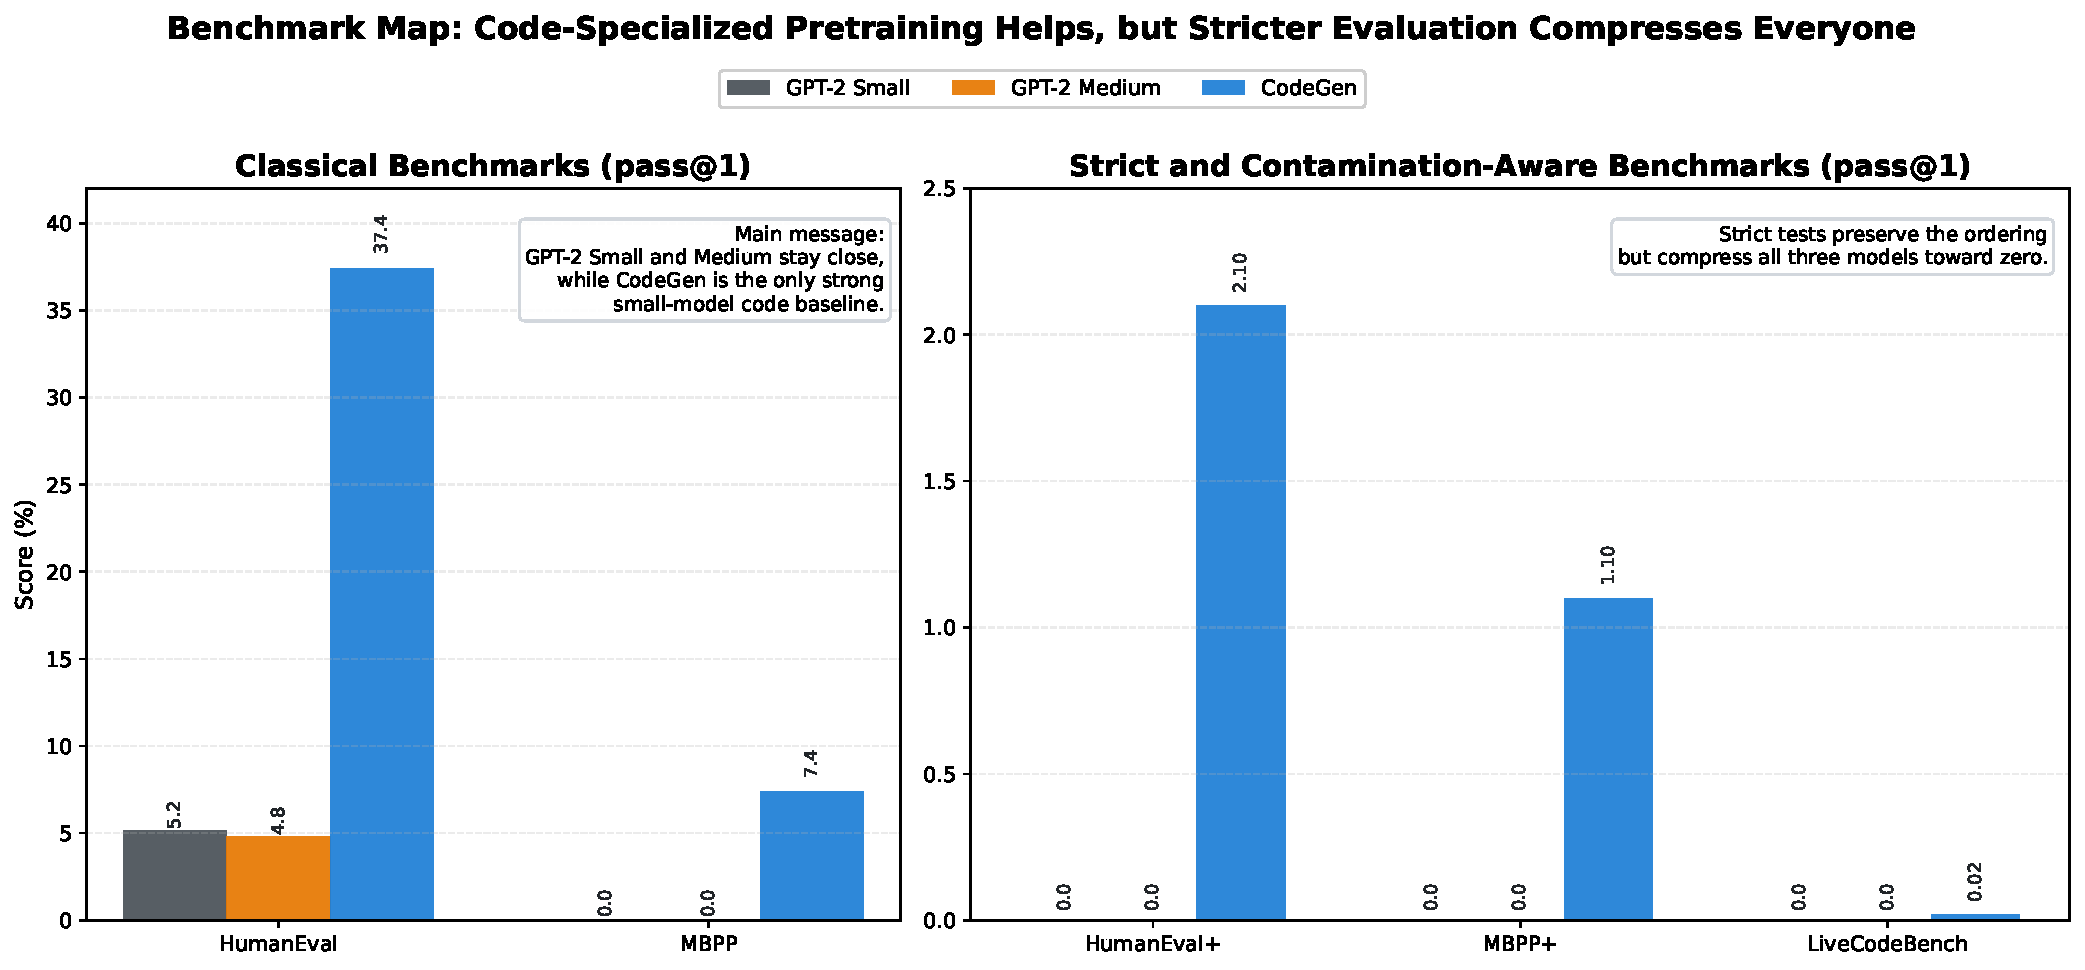
\includegraphics[width=\textwidth]{figure10_cross_benchmark_map.pdf}
\caption{Benchmark-wide comparison across classical, strict, and contamination-aware evaluations. HumanEval and MBPP show the main scale-versus-pretraining gap: GPT-2 Small and GPT-2 Medium remain close, while CodeGen is far stronger. Stricter benchmarks preserve the ranking but compress all three models sharply toward zero.}
\label{fig:benchmark_map}
\end{figure*}

Figure~\ref{fig:benchmark_map} summarizes the benchmark-wide pattern, while Table~\ref{tab:performance} presents the full HumanEval error-category totals:


\begin{table*}[t]
\centering
\caption{Model Performance on HumanEval (100 samples per problem; GPT-2 totals 16,400 attempts, while CodeGen has 16,300 scored attempts because \texttt{HumanEval/129} has no saved completions)}
\label{tab:performance}
\begin{tabular}{@{}lccccc@{}}
\toprule
\textbf{Model} & \textbf{Params} & \textbf{Success} & \textbf{Syntax} & \textbf{Runtime} & \textbf{Timeout} \\
\midrule
GPT-2 Small & 124M & 5.2 & 94.4 & 0.4 & 0.0 \\
GPT-2 Medium & 355M & 4.8 & 94.9 & 0.3 & 0.0 \\
CodeGen-350M & 350M & 37.4 & 61.1 & 1.1 & 0.3 \\
\bottomrule
\end{tabular}
\end{table*}

\textbf{Key observations:}

\begin{enumerate}
\item \textbf{Scaling does not yield a reliable gain}: GPT-2 Medium (355M parameters) achieves 4.8\% success versus GPT-2 Small (124M parameters) at 5.2\% success. This small numerical reversal is not statistically reliable, but it does contradict the simple expectation that added parameters should monotonically improve code-generation success.

\item \textbf{Pretraining explains more than scale in this comparison}: CodeGen-350M has nearly identical parameter count to GPT-2 Medium but achieves 7.8$\times$ higher success (37.4\% vs. 4.8\%), showing that parameter count alone does not explain the gap and that pretraining regime is the stronger explanation in this comparison~\cite{nijkamp2022codegen}.

\item \textbf{Failure modes differ across checkpoints}: GPT-2 models fail almost entirely on syntax (94.4-94.9\% of all generations), while CodeGen leaves a larger fraction of generations executable enough to surface runtime errors and occasional timeouts, suggesting a different executable-code profile in this comparison.

\item \textbf{Both GPT-2 scales fail similarly}: The near-identical error distributions between Small (94.4\% syntax) and Medium (94.9\% syntax) suggest they learned similar---and similarly inadequate---code representations despite 2.9$\times$ parameter difference.
\end{enumerate}

\subsection{Statistical Validation of the Scaling Paradox}

The raw percentages in Table~\ref{tab:performance} could still reflect task-level sampling noise, especially for the narrow 5.2\% vs. 4.8\% GPT-2 comparison. We therefore summarize problem-level bootstrap intervals and HumanEval pass@10 estimates in Table~\ref{tab:significance}.

\begin{table}[t]
\centering
\caption{Problem-Level Statistical Validation}
\label{tab:significance}
\scriptsize
\resizebox{\columnwidth}{!}{%
\begin{tabular}{@{}lcc@{}}
\toprule
\textbf{Model} & \textbf{Success \% [95\% CI]} & \textbf{pass@10 [95\% CI]} \\
\midrule
GPT-2 Small & 5.15 [4.49, 5.84] & 37.17 [33.50, 40.83] \\
GPT-2 Medium & 4.79 [3.94, 5.77] & 33.09 [29.55, 36.79] \\
CodeGen-350M & 37.42 [35.77, 39.13] & 97.90 [97.41, 98.36] \\
\bottomrule
\end{tabular}
}
\end{table}

\textbf{Finding}: The GPT-2 Small vs. GPT-2 Medium difference is not statistically reliable at the problem level (+0.37 percentage points, 95\% CI $[-0.73, 1.37]$, $p=0.5001$). By contrast, both GPT-2 models differ dramatically from CodeGen: GPT-2 Small vs. CodeGen is $-32.27$ points (95\% CI $[-34.06, -30.47]$, $p=0.0001$), and GPT-2 Medium vs. CodeGen is $-32.63$ points (95\% CI $[-34.57, -30.68]$, $p=0.0001$).

\textbf{Interpretation}: The scaling paradox within the GPT-2 family is therefore best understood as a \emph{failure to improve}, not as a confidently estimated reversal in favor of GPT-2 Small. The code-pretraining gap, however, is large, stable, and statistically unambiguous. Figure~\ref{fig:bootstrap_forest} makes the same contrast visible across both HumanEval and MBPP. For transparency, the saved bootstrap summary keeps all 164 CodeGen task IDs by treating the empty \texttt{HumanEval/129} entry as zero success, whereas the sample-level table above is based on the 163 tasks with scored completions; Appendix Figure~\ref{fig:coverage_audit} shows the final scored-vs-intended completion counts and the pre-sync repair burden for the repaired HumanEval artifacts.

\begin{figure*}[t]
\centering
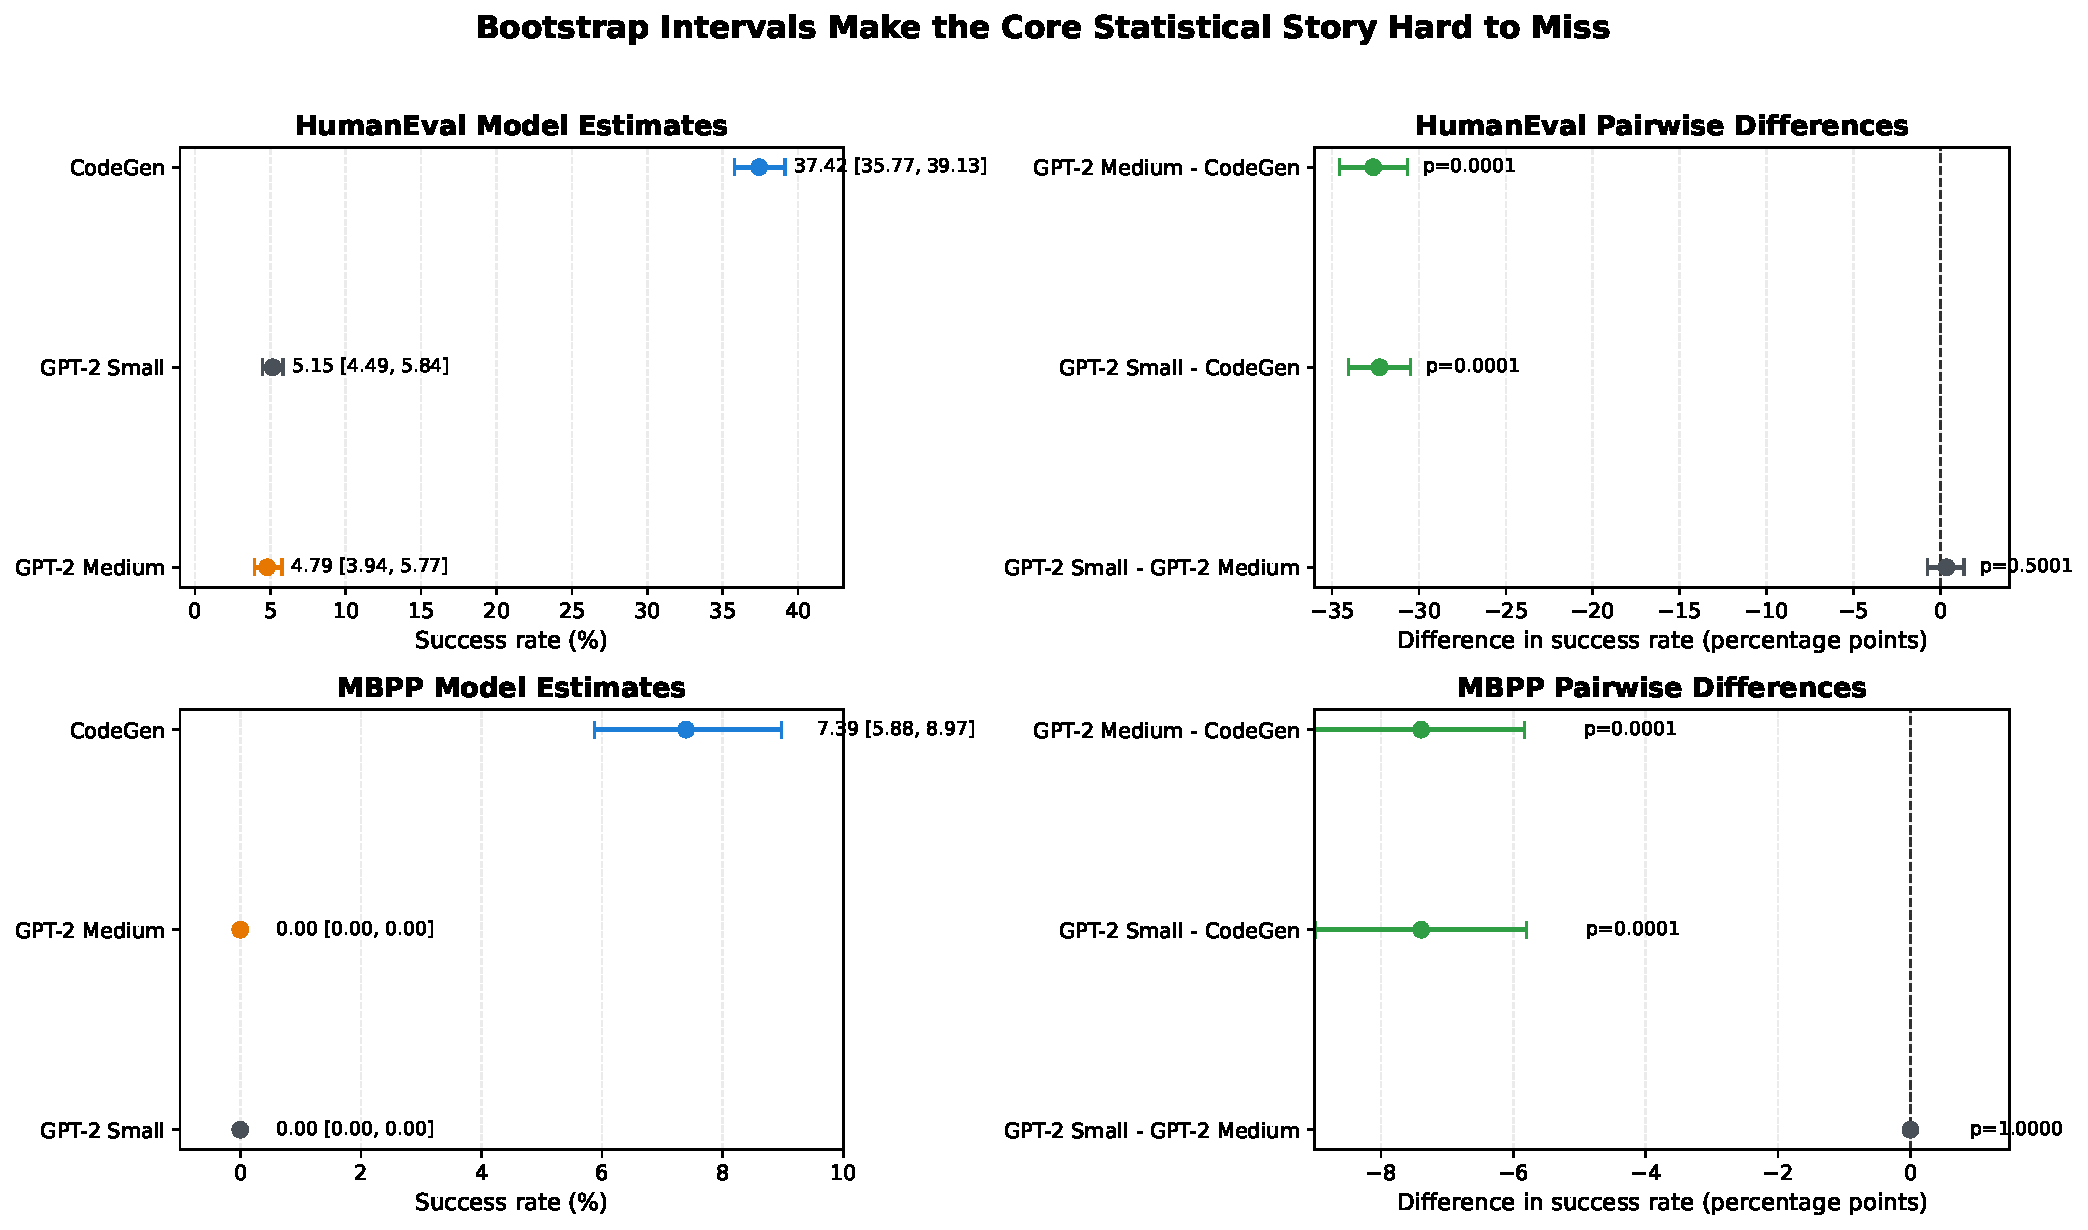
\includegraphics[width=\textwidth]{figure11_bootstrap_forest.pdf}
\caption{Bootstrap confidence intervals and pairwise success-rate deltas for the main HumanEval and MBPP comparisons. The GPT-2 Small / Medium gap overlaps zero on both benchmarks, whereas both GPT-2 models are cleanly separated from CodeGen.}
\label{fig:bootstrap_forest}
\end{figure*}

\subsection{External Validation on MBPP}

To test whether the scaling paradox is specific to HumanEval, we reran all three models on the full sanitized MBPP test split, using all 257 tasks and 20 samples per task. This gives a second benchmark with different prompt style and shorter programming tasks, while keeping the same Python execution setting.

\begin{table}[t]
\centering
\caption{Full-Coverage MBPP Validation}
\label{tab:mbpp_validation}
\scriptsize
\resizebox{\columnwidth}{!}{%
\begin{tabular}{@{}lcccc@{}}
\toprule
\textbf{Model} & \textbf{Success \% [95\% CI]} & \textbf{pass@5 [95\% CI]} & \textbf{Syntax \%} & \textbf{Runtime \%} \\
\midrule
GPT-2 Small & 0.00 [0.00, 0.00] & 0.00 [0.00, 0.00] & 96.30 & 0.54 \\
GPT-2 Medium & 0.00 [0.00, 0.00] & 0.00 [0.00, 0.00] & 98.31 & 0.18 \\
CodeGen-350M & 7.39 [5.88, 8.97] & 22.96 [18.95, 27.09] & 39.88 & 16.11 \\
\bottomrule
\end{tabular}
}
\end{table}

\textbf{Finding}: The scaling failure transfers cleanly. On MBPP, GPT-2 Small and GPT-2 Medium are tied at 0.0\% success, while CodeGen reaches 7.39\% success and 22.96\% pass@5. The pairwise bootstrap differences against CodeGen remain highly significant for both GPT-2 Small and GPT-2 Medium ($-7.39$ points in each case, $p=0.0001$), whereas GPT-2 Small vs. GPT-2 Medium is exactly 0.0 points ($p=1.0$).

\textbf{Interpretation}: This external validation matters because it shows that the central claim is not a HumanEval artifact. Across both benchmarks, scaling the general-language GPT-2 family fails to produce useful code-generation gains, while code-specific pretraining continues to produce a qualitatively different failure profile. MBPP makes this difference even starker: the GPT-2 models collapse almost entirely to syntax errors, whereas CodeGen preserves a much larger executable regime with mixed wrong-output and runtime failures.

\subsection{Strict Re-Evaluation on HumanEval+}

To test whether the main HumanEval ranking survives a stronger unit-test suite, we re-scored the first five saved HumanEval samples per task with HumanEval+, using the EvalPlus test augmentation. This gives a stricter completion-level pass@1 estimate without rerunning the full generation pipeline.

\begin{table}[t]
\centering
\caption{Strict HumanEval Re-scoring with HumanEval+}
\label{tab:humaneval_plus}
\scriptsize
\resizebox{\columnwidth}{!}{%
\begin{tabular}{@{}lcc@{}}
\toprule
\textbf{Model} & \textbf{HumanEval pass@1} & \textbf{HumanEval+ pass@1} \\
\midrule
GPT-2 Small & 0.00 & 0.00 \\
GPT-2 Medium & 0.00 & 0.00 \\
CodeGen-350M & 2.90 & 2.10 \\
\bottomrule
\end{tabular}
}
\end{table}

\textbf{Finding}: The stricter re-evaluation preserves the same ordering as the main benchmark comparison. Both GPT-2 variants remain at 0.0\% pass@1, while CodeGen retains nonzero performance even after the extra hidden tests reduce it from 2.9\% to 2.1\%.

\textbf{Interpretation}: This result matters because it rules out an easy objection that our main HumanEval ranking is driven only by weak original unit tests. The absolute pass@1 values are lower here because HumanEval+ is stricter and because we cap the re-score at five saved samples per task, but the relative conclusion is unchanged: scaling GPT-2 does not help, whereas code-specialized pretraining still produces measurably more robust completions.

\subsection{Strict Re-Evaluation on MBPP+}

We next evaluate MBPP+ with the official EvalPlus `mbpp' evaluator, reporting the Base+Extra score as our primary strict metric. Because MBPP+ is a versioned benchmark derived from MBPP-sanitized rather than the original MBPP split, we report it separately from Table~\ref{tab:mbpp_validation} and do not compare it directly to legacy MBPP numbers.

\begin{table}[t]
\centering
\caption{Strict MBPP+ Re-scoring with EvalPlus}
\label{tab:mbpp_plus}
\scriptsize
\resizebox{\columnwidth}{!}{%
\begin{tabular}{@{}lccc@{}}
\toprule
\textbf{Model} & \textbf{Tasks} & \textbf{MBPP+ pass@1} & \textbf{MBPP+ pass@10} \\
\midrule
GPT-2 Small & 378 & 0.00 & 0.00 \\
GPT-2 Medium & 378 & 0.00 & 0.00 \\
CodeGen-350M & 378 & 1.10 & 6.40 \\
\bottomrule
\end{tabular}
}
\end{table}

\textbf{Finding}: The stricter MBPP+ evaluation preserves the same qualitative ordering as the full MBPP benchmark. Both GPT-2 variants remain at 0.0\% under the stronger Base+Extra score, while CodeGen retains 1.1\% pass@1 and 6.4\% pass@10.

\textbf{Interpretation}: MBPP+ strengthens the negative claim and slightly narrows the positive one. The GPT-2 scaling failure survives a stricter, versioned test suite, while CodeGen remains the only model with nonzero strict performance. At the same time, the lower absolute numbers emphasize that even CodeGen's advantage on small-model code generation is fragile under stronger hidden tests.

\subsection{Contamination-Aware Validation on LiveCodeBench}

To test whether the same ranking survives on a newer contamination-aware benchmark, we evaluated all three models on LiveCodeBench release v2~\cite{jain2024livecodebench} in its default code-generation-lite setting, using 10 samples per task. This benchmark is substantially harder than HumanEval or MBPP for models in the 124M--355M range.

\begin{table}[t]
\centering
\caption{LiveCodeBench release v2 Validation}
\label{tab:livecodebench_validation}
\scriptsize
\resizebox{\columnwidth}{!}{%
\begin{tabular}{@{}lcccc@{}}
\toprule
\textbf{Model} & \textbf{Tasks scored} & \textbf{pass@1 \%} & \textbf{pass@5 \%} & \textbf{pass@10 \%} \\
\midrule
GPT-2 Small & 510 & 0.00 & 0.00 & 0.00 \\
GPT-2 Medium & 511 & 0.00 & 0.00 & 0.00 \\
CodeGen-350M & 511 & 0.02 & 0.10 & 0.20 \\
\bottomrule
\end{tabular}
}
\end{table}

\textbf{Finding}: The relative ordering is preserved, but the absolute performance landscape changes sharply. GPT-2 Small and GPT-2 Medium remain exactly at zero, while CodeGen is only marginally nonzero. For GPT-2 Small, one task did not yield a valid scored record under the custom export path, so pass@k is reported over 510 scored tasks; the other two models are scored over the full 511 tasks.

\textbf{Interpretation}: LiveCodeBench is therefore best read as a calibration result rather than a new positive benchmark win. It strengthens the negative claim that scale alone does not induce useful code generation in small general-language models, while also showing that a 350M code-pretrained model is still far from practically capable on a harder contamination-aware benchmark. The main positive CodeGen advantage is strongest on the classical Python benchmarks (HumanEval and MBPP), not on this harsher stress test. Appendix Figure~\ref{fig:strictness_cascade} shows the same compression as a pass@1 cascade across benchmark families.

\subsection{Within-Family Continued-Pretraining Control in CodeGen}

To reduce the objection that GPT-2 versus CodeGen is ``just a family difference,'' we evaluate the CodeGen-350M NL$\rightarrow$Multi$\rightarrow$Mono checkpoint ladder described by \citet{nijkamp2022codegen}. This comparison holds architecture and parameter count fixed while changing the added continued-pretraining corpus. We treat it as a strong within-family control, not as a pure distribution-only isolation, because later checkpoints also receive additional optimization steps and tokens.

\begin{table}[t]
\centering
\caption{CodeGen-350M Continued-Pretraining Ladder}
\label{tab:codegen_ladder}
\scriptsize
\resizebox{\columnwidth}{!}{%
\begin{tabular}{@{}lccc@{}}
\toprule
\textbf{Checkpoint} & \textbf{HumanEval tasks} & \textbf{HumanEval success \%} & \textbf{MBPP success \%} \\
\midrule
CodeGen-NL & 164 & 31.60 & 0.02 \\
CodeGen-Multi & 164 & 30.66 & 1.23 \\
CodeGen-Mono & 164 & 39.00 & 2.76 \\
\bottomrule
\end{tabular}
}
\end{table}

\textbf{Finding}: Mono is strongest on both benchmarks, but the ladder behaves differently across them. On full-coverage HumanEval, Mono significantly exceeds both NL (39.00\% vs.\ 31.60\%, $p=0.0001$) and Multi (39.00\% vs.\ 30.66\%, $p=0.0001$), while NL vs.\ Multi is small and not significant (31.60\% vs.\ 30.66\%, $p=0.4421$). On MBPP, the ladder remains cleanly monotone: NL reaches 0.02\%, Multi 1.23\%, and Mono 2.76\%, with significant improvements from NL to Multi ($p=0.0001$) and Multi to Mono ($p=0.0157$).

\textbf{Interpretation}: This is now stronger within-family evidence because the HumanEval ladder is full-coverage rather than OOM-truncated. Even so, the HumanEval ladder is still mixed at the intermediate checkpoint because Multi does not improve over NL, and the checkpoints still differ in additional compute and curriculum. We therefore use the ladder to support a continued-pretraining plus curriculum claim, not a matched-compute law. The MBPP result is cleaner and supports the narrower claim that continued-pretraining plus curriculum effects materially improve small-model code generation within a single family.

As an auxiliary diagnostic, prompt perplexity on the ladder prompts is lowest for Mono on both HumanEval (4.87) and MBPP (4.46), intermediate for NL (4.93 and 4.64), and highest for Multi (5.54 and 5.23). Following CodeGen, we interpret these numbers only as prompt--checkpoint compatibility diagnostics, not as direct explanations of functional gains, so they remain secondary evidence rather than a main result.

Figure~\ref{fig:codegen_ladder_benchmarks} visualizes the key asymmetry: HumanEval only improves decisively at the final Mono stage, whereas MBPP improves throughout the ladder.

\begin{figure*}[t]
\centering
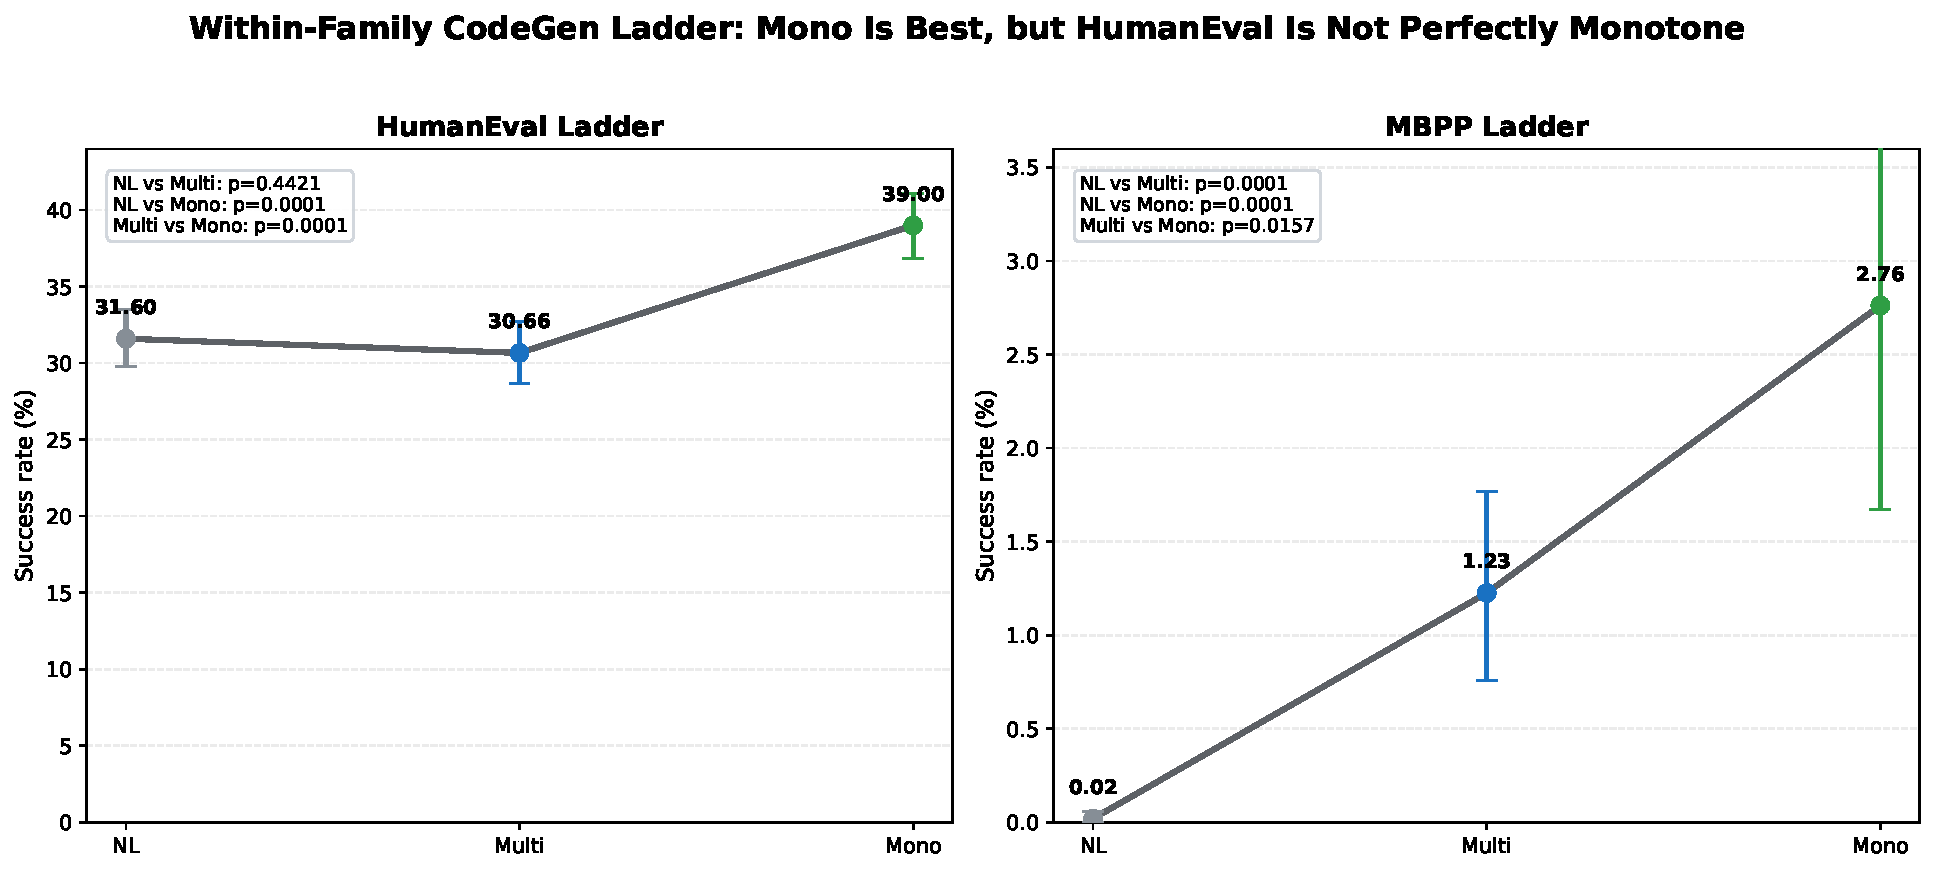
\includegraphics[width=\textwidth]{figure12_codegen_ladder_benchmarks.pdf}
\caption{Within-family CodeGen ladder performance on HumanEval and MBPP. Mono is best on both benchmarks, but only MBPP is cleanly monotone at the intermediate Multi checkpoint. HumanEval improves decisively only at the final Mono stage.}
\label{fig:codegen_ladder_benchmarks}
\end{figure*}

\subsection{Prompt and Decoding Robustness Controls}

The preceding results show that parameter count and pretraining distribution are not interchangeable. We next ask a more systems-oriented question: how much of the observed reliability depends on the surrounding generation protocol? We therefore ran targeted robustness controls on the three most informative small models: GPT-2 Medium, CodeGen-Mono 350M, and Qwen2.5-Coder 0.5B. These controls are not intended to replace the larger 100-sample main sweeps; they are sensitivity analyses using fixed saved artifacts, 20 samples per HumanEval task, and 10 samples per MBPP task.

Figure~\ref{fig:targeted_robustness_controls} summarizes the result. Prompt format has a large effect on HumanEval for code-specialized models: CodeGen-Mono moves from 42.6\% sample success under signature-only prompting to 71.2\% under comment-plus-signature prompting, while Qwen2.5-Coder moves from 41.6\% under canonical prompting to 54.7\% under comment-plus-signature prompting. GPT-2 Medium remains weak across all prompt styles, ranging only from 1.1\% to 2.1\% sample success, so prompt format does not rescue the general-language model's syntax bottleneck.

Decoding temperature has a different profile. On HumanEval, GPT-2 Medium improves slightly at high temperature (3.1\% vs.\ 2.1\% standard), but remains far below the code-specialized models. CodeGen-Mono is strongest at standard temperature (56.1\% sample success), and Qwen2.5-Coder is slightly strongest at low temperature (42.2\%) but loses distinct-task coverage relative to standard decoding. On MBPP, low temperature improves sample success for both CodeGen-Mono (14.4\% vs.\ 8.6\% standard) and Qwen2.5-Coder (28.8\% vs.\ 19.0\% standard), but it reduces distinct-task coverage: CodeGen-Mono falls from 34.2\% covered tasks under standard decoding to 30.7\% under low temperature, and Qwen2.5-Coder falls from 54.9\% to 49.8\%.

\textbf{Interpretation}: These controls strengthen the systems framing. The bottleneck is not parameter count alone, and not even pretraining alone. Code-generation reliability also depends on prompt interface, decoding policy, benchmark distribution, and the metric chosen to summarize output. MBPP makes the tradeoff especially clear: an intervention can increase the number of successful samples while reducing the number of distinct problems for which the model finds any solution.

\begin{figure*}[t]
\centering
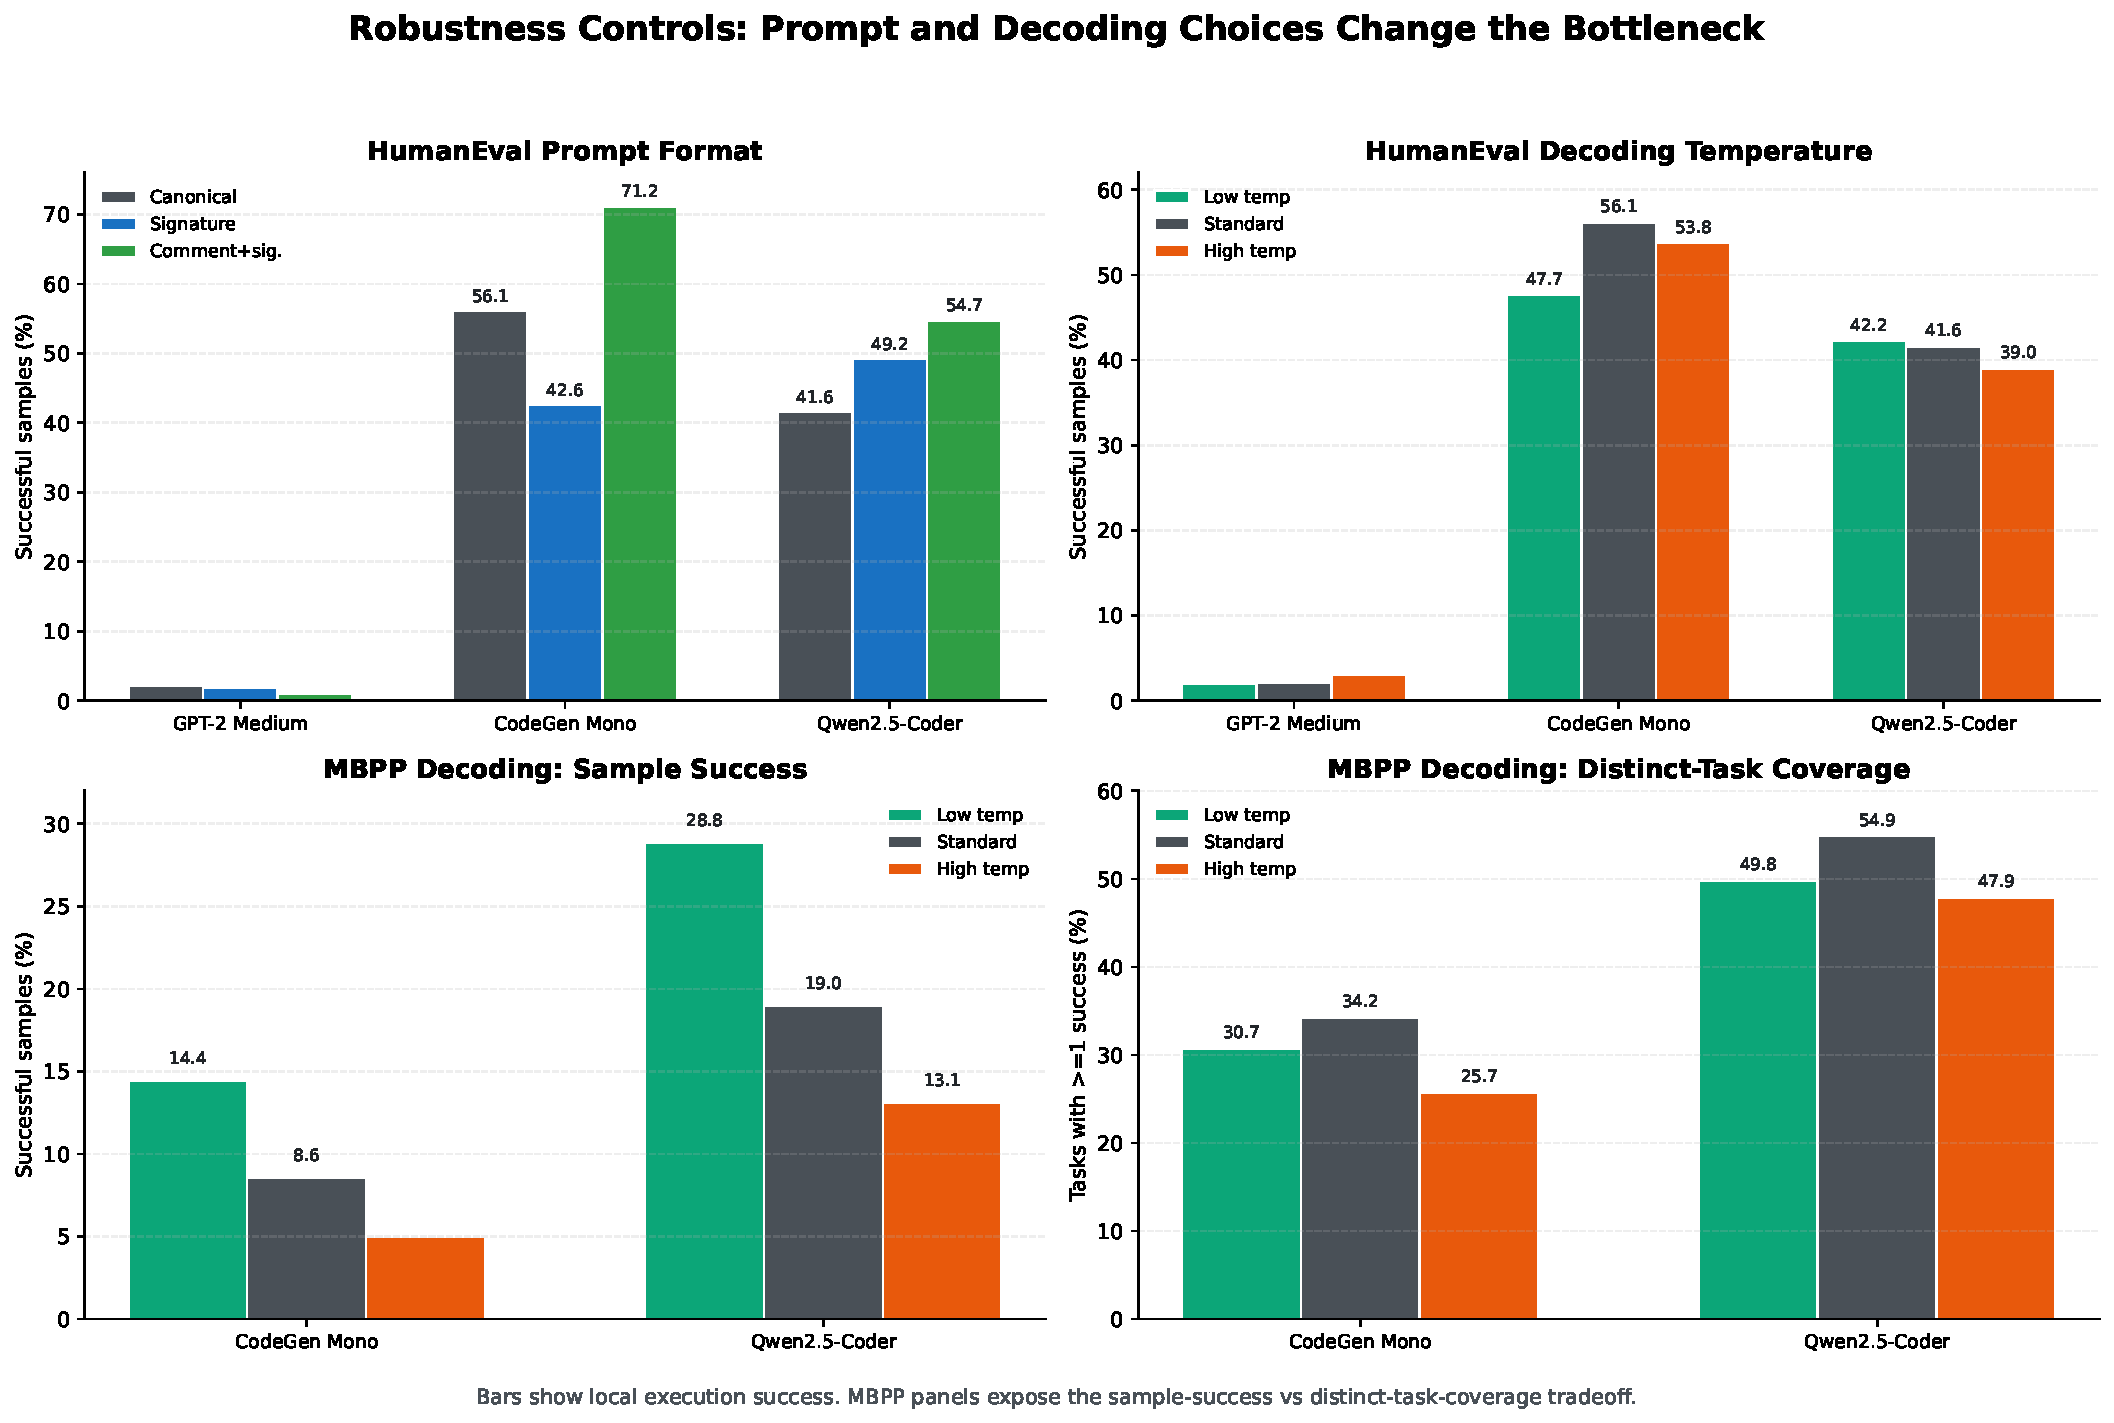
\includegraphics[width=\textwidth]{figure15_targeted_robustness_controls.pdf}
\caption{Targeted prompt and decoding robustness controls. Prompt format strongly changes HumanEval sample success for CodeGen-Mono and Qwen2.5-Coder while leaving GPT-2 Medium near zero. Decoding temperature is model- and benchmark-specific. On MBPP, low temperature increases repeated sample success but reduces distinct-task coverage, showing that aggregate success and reliability across tasks can move in opposite directions.}
\label{fig:targeted_robustness_controls}
\end{figure*}

\subsection{Scaled Follow-Ups on CodeGen Ladder Signature Layers}

To test whether the ladder's signature layers also show graded behavior, we ran a final 20-problem / 10-sample scaled-ablation follow-up on CodeGen-NL layer 11, CodeGen-Multi layer 7, and CodeGen-Mono layer 13 using scales $\{0.75, 0.5, 0.25, 0.0\}$.

\begin{table}[t]
\centering
\caption{Scaled Follow-Ups on CodeGen Ladder Signature Layers}
\label{tab:codegen_ladder_scaled}
\scriptsize
\resizebox{\columnwidth}{!}{%
\begin{tabular}{@{}lcccc@{}}
\toprule
\textbf{Checkpoint} & \textbf{Layer} & \textbf{Baseline} & \textbf{0.25 scale} & \textbf{0.0 scale} \\
\midrule
CodeGen-NL & 11 & 25.5 & 8.5 & 17.0 \\
CodeGen-Multi & 7 & 41.0 & 1.0 & 61.5 \\
CodeGen-Mono & 13 & 31.0 & 2.0 & 29.0 \\
\bottomrule
\end{tabular}
}
\end{table}

\textbf{Finding}: Two of the three ladder follow-ups are mechanistically useful. In CodeGen-NL, layer 11 degrades in the expected direction under attenuation (25.5\% $\rightarrow$ 22.5\% $\rightarrow$ 16.0\% $\rightarrow$ 8.5\%), indicating that the earlier checkpoint relies on a comparatively brittle syntactic support layer. In CodeGen-Mono, layer 13 preserves 33.5\% success at scale 0.75, falls to 2.0\% at scale 0.25, and still retains 29.0\% success under full zeroing while shifting 22.5\% of outputs into runtime errors, reinforcing the main claim that later code-pretrained checkpoints retain a broader executable-code regime. CodeGen-Multi is less clean: layer 7 behaves plausibly under partial attenuation, but full zeroing unexpectedly improves success to 61.5\%, so we treat that leg as anomalous and exclude it from the mechanistic claim.

\textbf{Interpretation}: These follow-ups strengthen the ladder interpretation without making it artificially cleaner than the evidence. The NL checkpoint looks more like a syntax-dependent intermediate stage, while the Mono checkpoint again shows the mixed residual/runtime behavior that marks distributed executable-code support in the main CodeGen analysis. The anomalous Multi zero-ablation result prevents us from claiming a simple monotone mechanistic progression across the whole ladder, but it does not erase the broader pattern that later continued-pretraining stages can change both benchmark performance and the layerwise failure geometry of code generation.

\begin{figure*}[t]
\centering
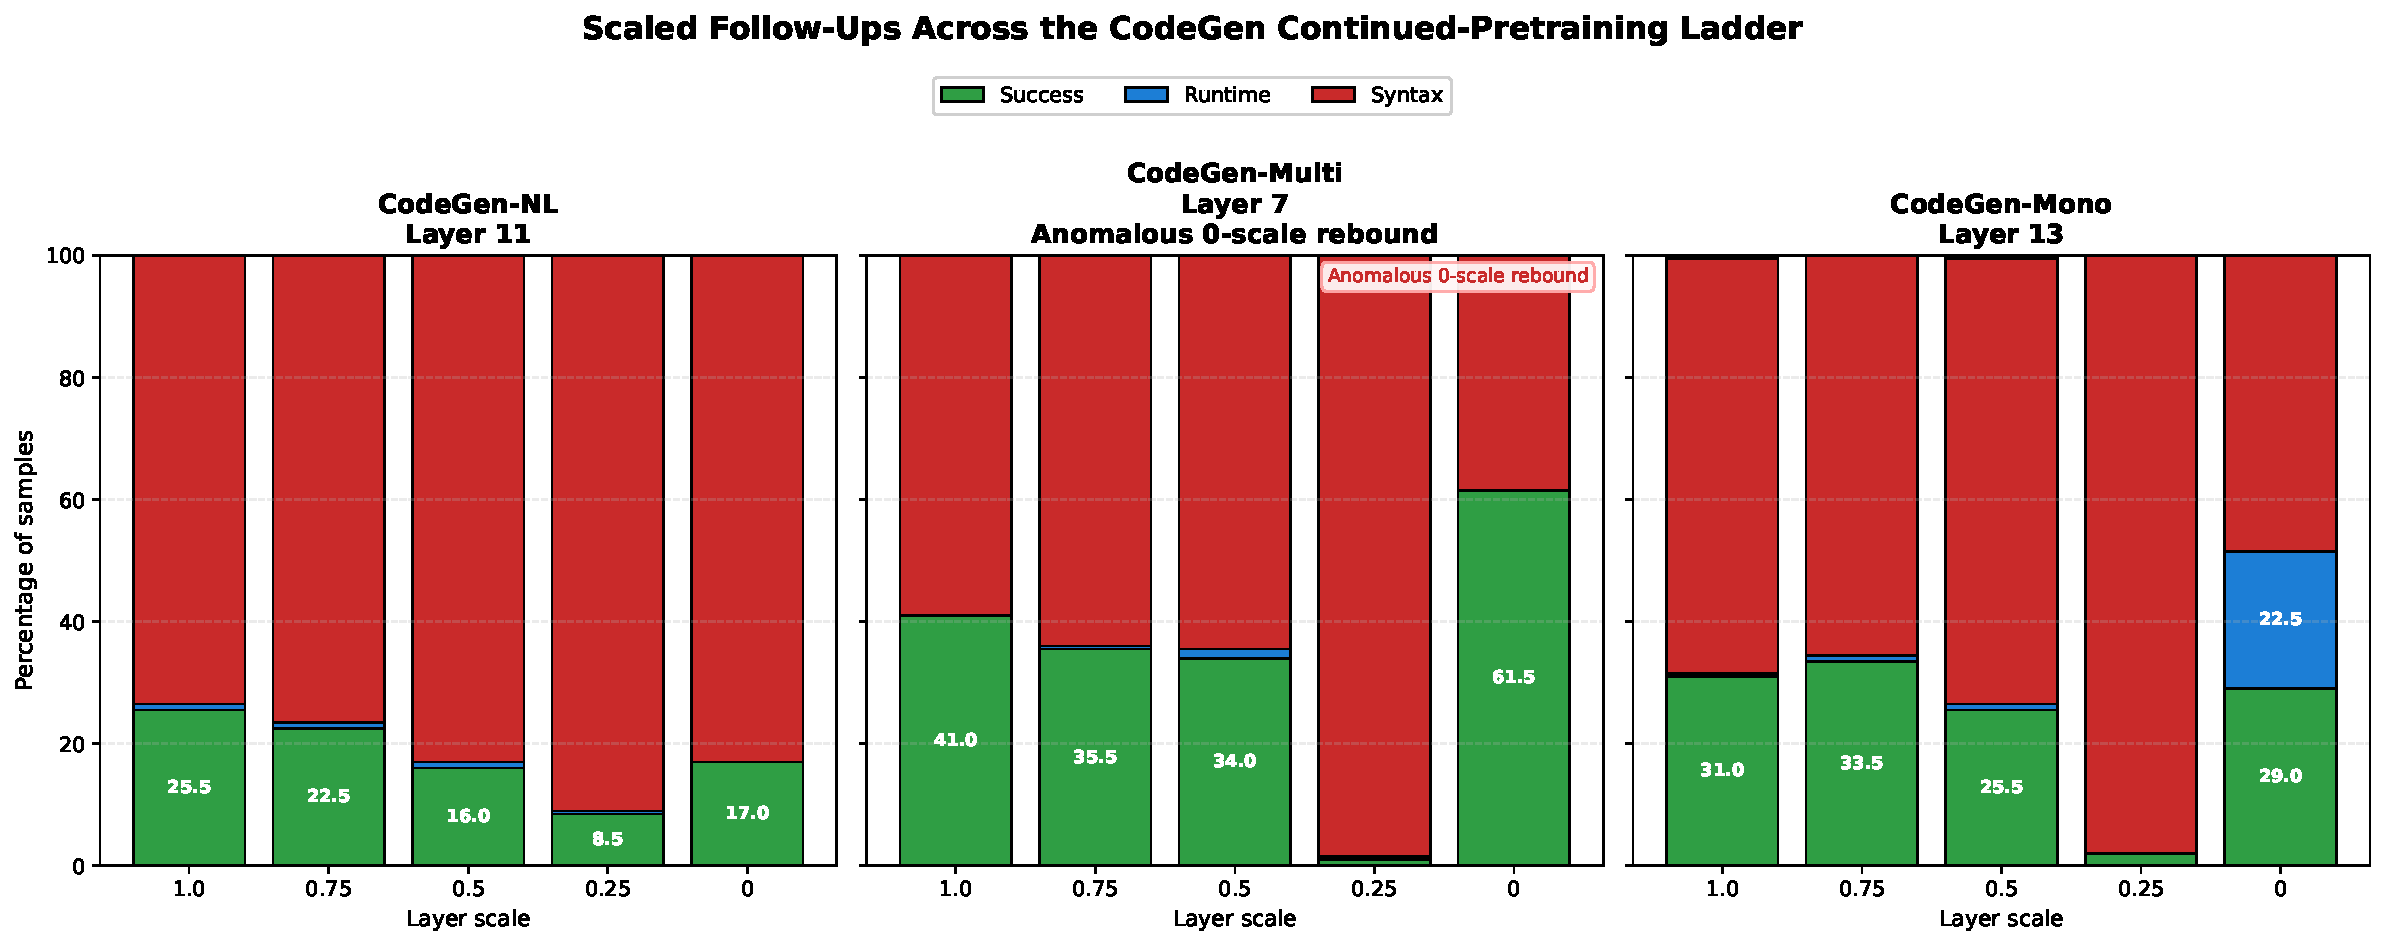
\includegraphics[width=\textwidth]{figure8_codegen_ladder_followups.pdf}
\caption{Scaled follow-up interventions on signature layers from the CodeGen continued-pretraining ladder. CodeGen-NL layer 11 degrades toward syntax collapse under attenuation, CodeGen-Mono layer 13 reopens a mixed executable/runtime regime under full zeroing, and CodeGen-Multi layer 7 is anomalous at 0.0 scale. We therefore use the NL and Mono legs as the clean within-family mechanistic evidence.}
\label{fig:codegen_ladder_followups}
\end{figure*}

\subsection{Layer Ablation Reveals Distinct Failure Profiles}

To understand \emph{why} scaling fails for GPT-2 but succeeds for CodeGen, we ablate each layer individually and measure the impact on code generation success.

\begin{figure}[t]
\centering
\includegraphics[width=0.9\columnwidth]{figure2_ablation_heatmap.png}
\caption{Single-layer zeroing across the three models. GPT-2 Medium falls to 0\% success for every layer, with layer 12 standing out only through a runtime-error shift, whereas CodeGen retains several nonzero layers. The contrast is narrow brittleness versus broader residual support, not robustness versus no effect.}
\label{fig:ablation_heatmap}
\end{figure}

\begin{table*}[t]
\centering
\caption{Signature Ablation Layers and Failure Modes}
\label{tab:critical_layers}
\footnotesize
\setlength{\tabcolsep}{4pt}
\resizebox{\textwidth}{!}{%
\begin{tabular}{@{}lcccc@{}}
\toprule
\textbf{Model} & \textbf{Total Layers} & \textbf{Signature Layer(s)} & \textbf{Residual Success} & \textbf{Failure Signature (Ablated)} \\
\midrule
GPT-2 Small & 12 & Layer 2 (17\%) & 1.8\% & 98.2\% syntax \\
GPT-2 Medium & 24 & Layer 12 (50\%) & 0.0\% & 76.1\% syntax, 23.9\% runtime \\
CodeGen-350M & 20 & Layers 5, 7, 13, 18 & 11.7\%, 4.6\%, 29.5\%, 0.1\% & Mostly syntax; layer 13 adds 18.9\% runtime \\
\bottomrule
\end{tabular}
}
\end{table*}

\textbf{Key findings:}

\begin{enumerate}
\item \textbf{GPT-2 Medium is uniformly brittle under full-layer ablation}: every single-layer ablation reduces success to 0\%, so the model does not exhibit residual robustness anywhere in depth.

\item \textbf{Layer 12 is distinguished by failure mode, not residual success}: when layer 12 is ablated, GPT-2 Medium produces 23.9\% runtime errors instead of collapsing entirely to syntax errors. No other medium layer shows this pattern.

\item \textbf{CodeGen retains partial survival in several layers}: layers 5, 7, 13, and 18 all preserve nonzero success when ablated, with layer 13 preserving 29.5\% success. This is still a harsh failure regime, but it is broader than either GPT-2 variant.

\item \textbf{Residual robustness and signature depth move together in this three-model snapshot}: GPT-2 Small's only surviving layer appears early (17\%), GPT-2 Medium's distinctive runtime-shift layer appears at mid depth (50\%), and CodeGen's strongest residual layer appears later (65\%). We treat this as descriptive evidence rather than a general law.
\end{enumerate}

\begin{figure*}[t]
\centering
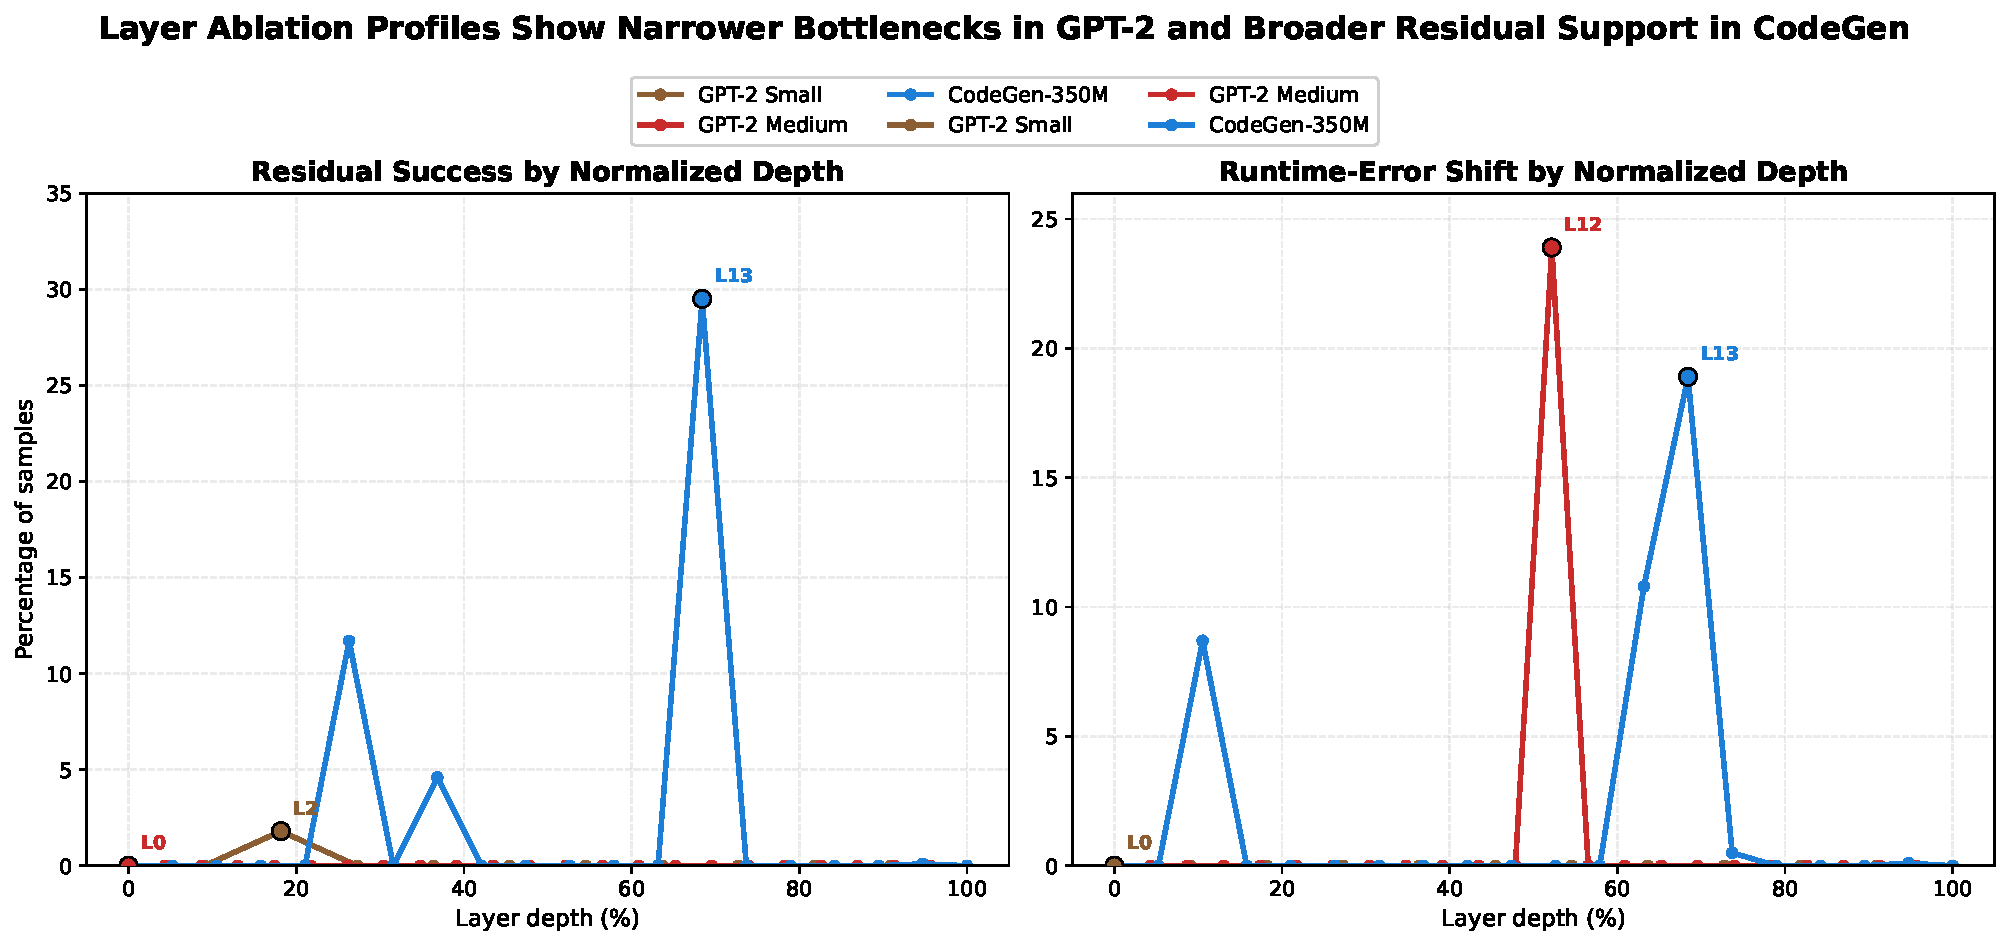
\includegraphics[width=\textwidth]{figure9_ablation_depth_profiles.pdf}
\caption{Normalized-depth view of the same ablations. GPT-2 Medium shows a narrow mid-depth runtime-shift spike without residual success, while CodeGen preserves both later residual success and a mixed executable/runtime regime centered on layer 13. This view isolates the mechanistic contrast more clearly than the heatmap alone.}
\label{fig:ablation_depth_profiles}
\end{figure*}

\subsection{Syntax Error Breakdown Reveals Distinct Failure Profiles}

To compare syntax-error profiles across checkpoints, we categorize the types of syntax errors each model produces.

\begin{table}[t]
\centering
\caption{Syntax Error Distribution by Type (\% of all syntax errors)}
\label{tab:syntax_errors}
\scriptsize
\setlength{\tabcolsep}{2pt}
\begin{tabular}{lcccccc}
\toprule
\textbf{Model} & \textbf{Ind.} & \textbf{Brack.} & \textbf{Quote} & \textbf{Kwd} & \textbf{Colon} & \textbf{Other} \\
\midrule
GPT-2 Small & 22.0 & 6.5 & 7.9 & 8.6 & 0.3 & 54.4 \\
GPT-2 Medium & 28.7 & 3.0 & 8.0 & 8.1 & 0.3 & 51.7 \\
CodeGen-350M & 7.4 & 23.1 & 5.3 & 2.4 & 4.7 & 57.0 \\
\bottomrule
\end{tabular}
\end{table}

\begin{figure}[t]
\centering
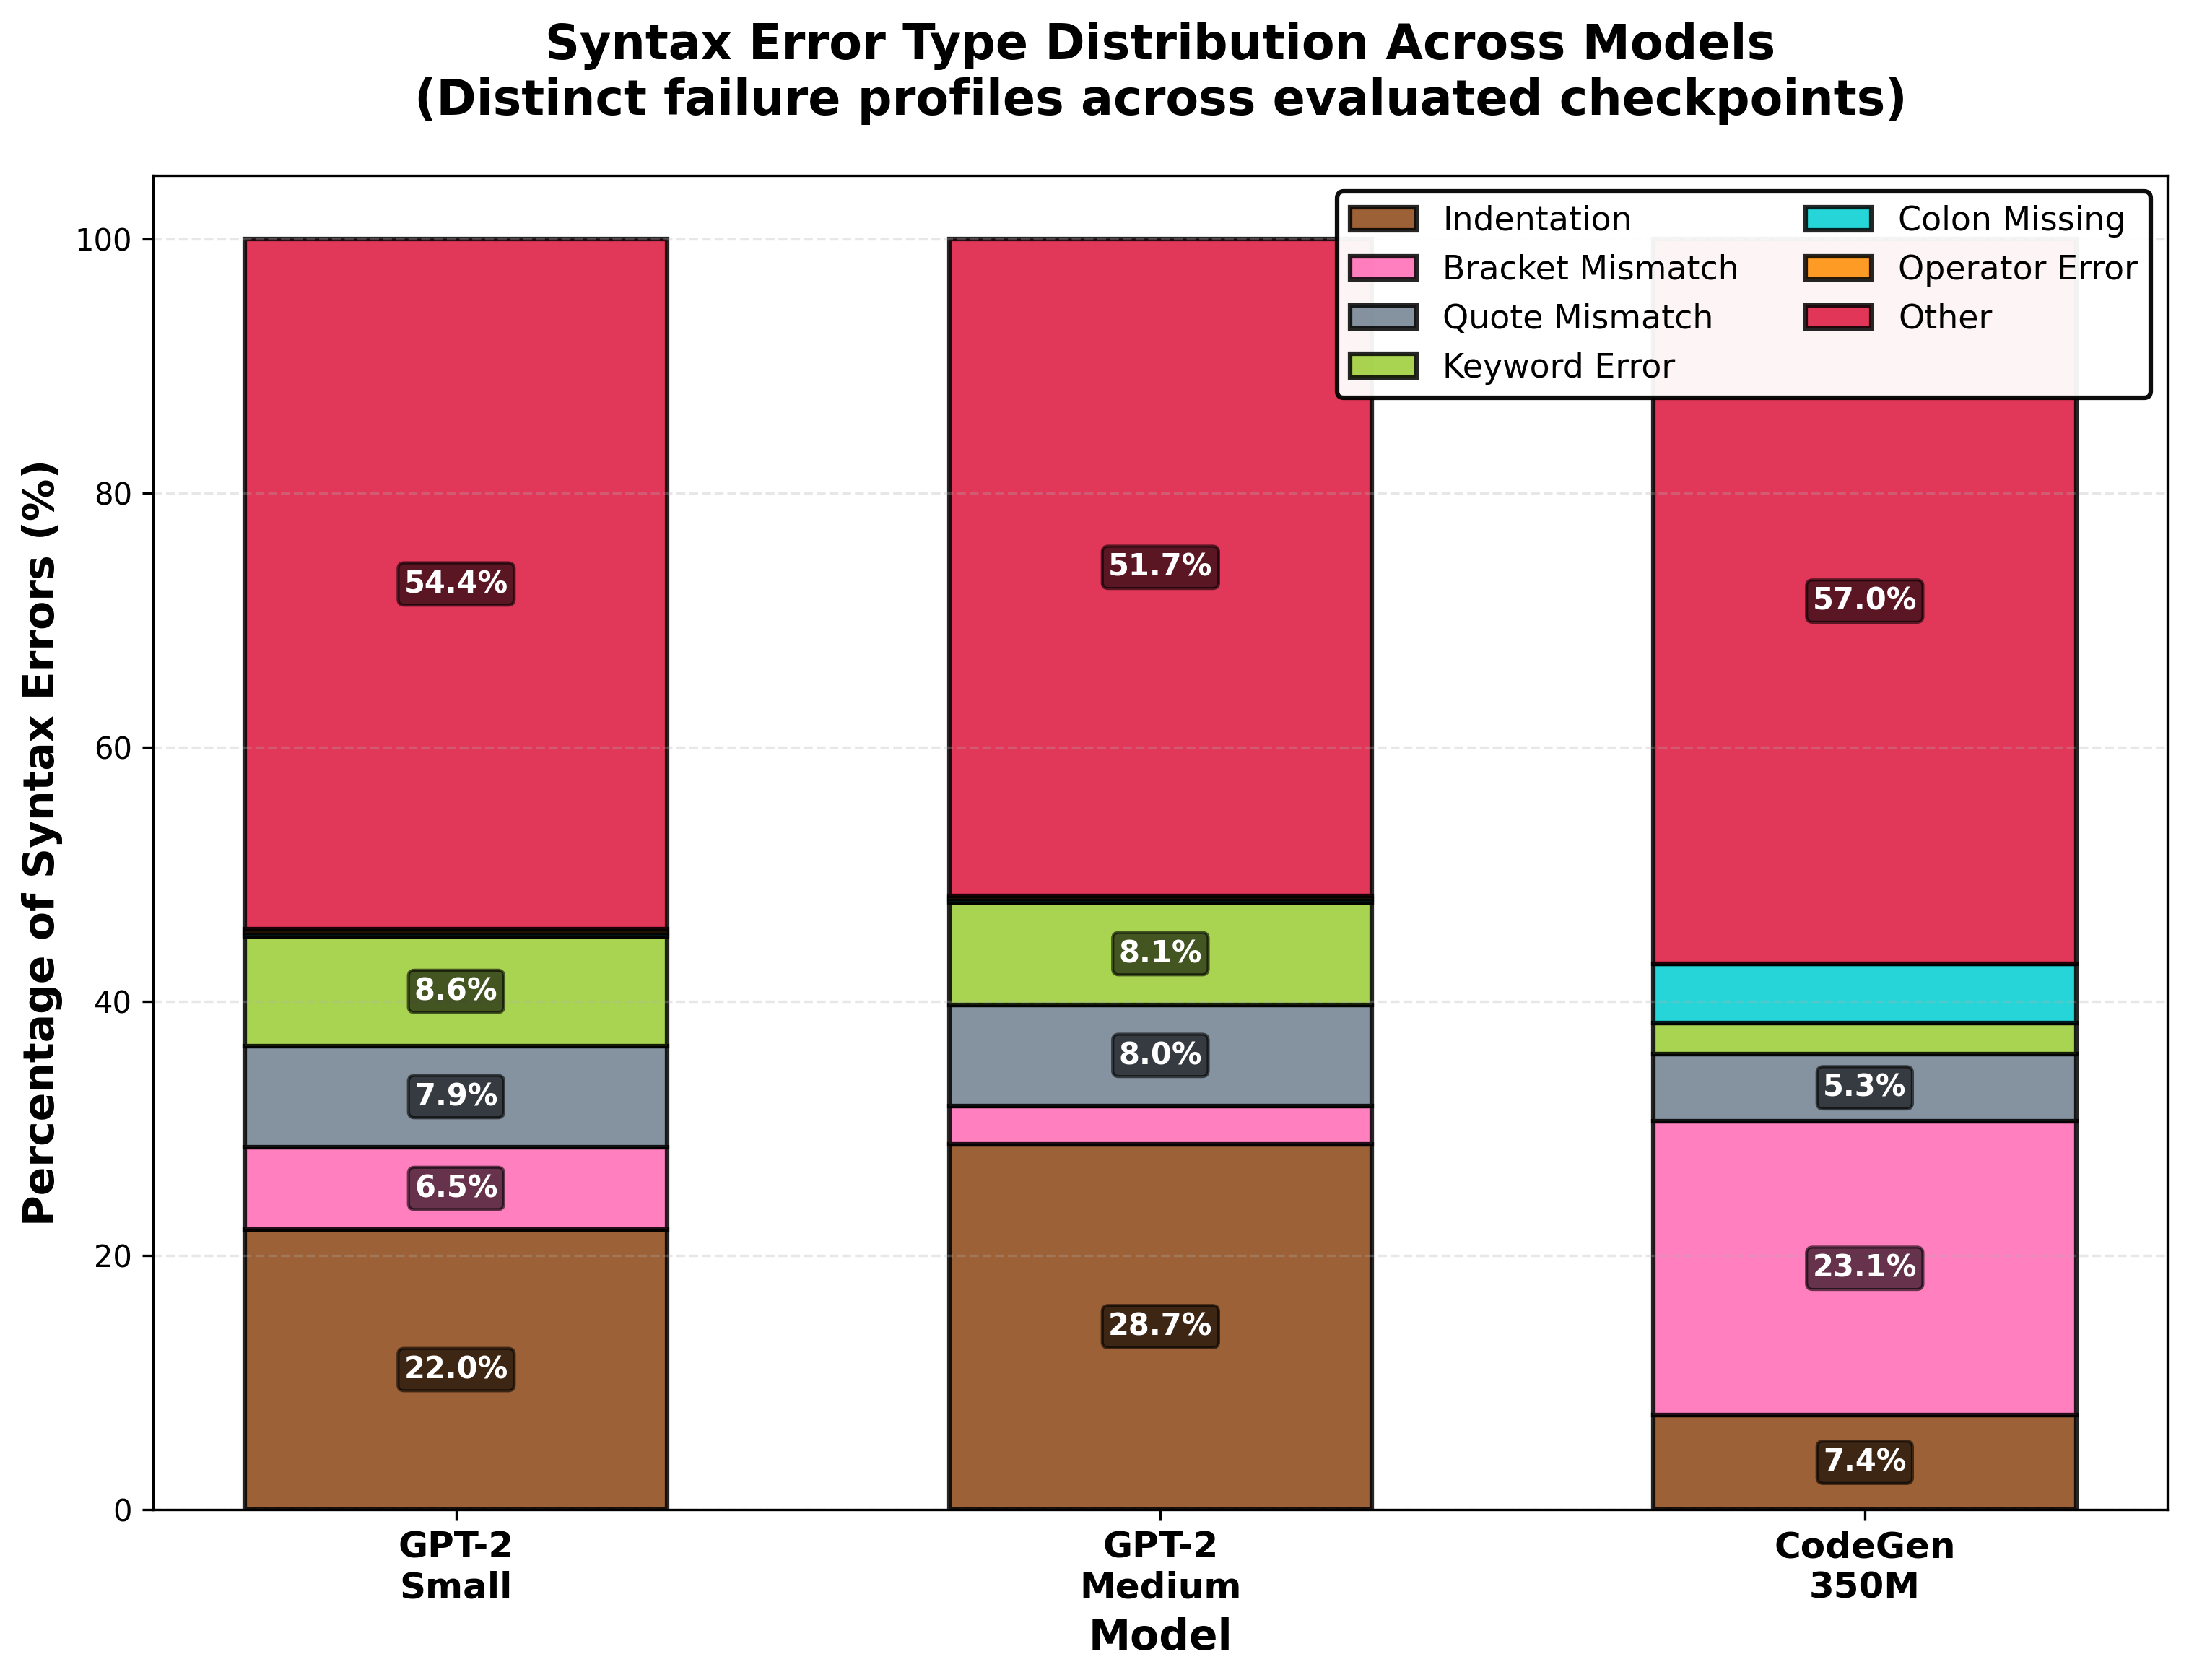
\includegraphics[width=0.9\columnwidth]{figure3_error_distribution.png}
\caption{Syntax-error profile by model. GPT-2 errors are dominated by indentation, whereas CodeGen shifts toward bracket mismatches. The difference is consistent with distinct syntactic priors across the evaluated checkpoints, but the error profile alone does not identify the training-data cause.}
\label{fig:error_distribution}
\end{figure}

\textbf{Key patterns:}

\begin{enumerate}
\item \textbf{GPT-2 struggles with indentation}: Both GPT-2 models produce 22-29\% indentation errors---far more than CodeGen (7.4\%). This pattern is consistent with weaker indentation handling in the two GPT-2 checkpoints under our evaluation, but our experiments do not isolate why that difference arises.

\item \textbf{Medium's indentation errors increase with scale}: GPT-2 Medium (28.7\%) produces more indentation errors than Small (22.0\%), showing that the larger GPT-2 checkpoint does not reduce this failure mode in our setting.

\item \textbf{CodeGen fails on brackets}: CodeGen produces 23.1\% bracket errors---more than 7$\times$ GPT-2 Medium's 3.0\%. One plausible interpretation is that its broader code pretraining, which includes substantial Java and C++ proportions~\cite{nijkamp2022codegen}, shapes this profile. Our experiments, however, do not isolate training-data composition as the cause of the bracket-error gap.

\item \textbf{Keyword and quote errors are similar}: All models produce 5-8\% quote errors and 2-9\% keyword errors, suggesting that these categories are not the main source of the observed cross-model contrast in this sample.

\item \textbf{`Other'' errors dominate}: 52--60\% of syntax errors fall outside our six main categories, indicating long-tailed failure modes (invalid operators, malformed imports, incorrect statement structure) that remain outside this coarse taxonomy.
\end{enumerate}

\subsection{Activation Analysis: A Compact Probe Signal at Layer 12}

To understand the mechanistic basis of GPT-2 Medium's distinctive layer-12 failure mode, we analyze which activation dimensions discriminate between successful and syntactically invalid generations.

\textbf{Methodology}: For 200 balanced samples (100 success, 100 syntax error), we mean-pool the hidden states $h_{12} \in \mathbb{R}^{1024}$ from transformer block 12 and compute dimension-wise difference magnitudes:

\begin{equation}
\Delta_i = | \text{mean}(h_{12,i}^{\text{success}}) - \text{mean}(h_{12,i}^{\text{failure}}) |
\end{equation}

\textbf{Finding}: The strongest probe dimensions are 121, 346, 615, 820, and 169. A logistic regression probe on these five coordinates reaches 72.5\% held-out accuracy, compared with 75.0\% for the full-layer probe and 67.5\% for the top-two-dimensional projection used in Figure~\ref{fig:activation_projection}.

\begin{table}[t]
\centering
\caption{Top Discriminative Dimensions in Layer 12}
\label{tab:dimensions}
\footnotesize
\setlength{\tabcolsep}{4pt}
\resizebox{\columnwidth}{!}{%
\begin{tabular}{ccccc}
\toprule
\textbf{Dim} & \textbf{Mean (S)} & \textbf{Mean (F)} & \textbf{Diff.} & \textbf{\% Sig.} \\
\midrule
121 & $-35.27$ & $-29.54$ & 5.73 & 0.90\% \\
346 & 17.03 & 14.19 & 2.84 & 0.44\% \\
615 & 6.96 & 4.21 & 2.75 & 0.43\% \\
820 & $-3.15$ & $-0.76$ & 2.39 & 0.37\% \\
169 & $-3.36$ & $-1.02$ & 2.34 & 0.37\% \\
\textbf{Remaining 1019 dims} & --- & --- & --- & \textbf{97.49\%} \\
\bottomrule
\end{tabular}
}
\end{table}

\textbf{Key observations:}

\begin{enumerate}
\item \textbf{A compact probe nearly matches the full layer}: The top-5 probe reaches 72.5\% accuracy, which is 96.7\% of the full-layer probe's 75.0\% accuracy.

\item \textbf{The signal is compact but not exclusive}: The same five dimensions account for only 2.51\% of the total absolute mean shift, so much of the layer still moves between successful and failed generations even though a small probe captures most linear separability.

\item \textbf{Dimension 121 dominates the mean gap}: It shows a 5.73-unit difference between successful and failed generations, while the other top coordinates contribute smaller but consistent shifts.

\item \textbf{The 2D view is only partially separable}: The top-two-dimensional projection reaches 67.5\% held-out accuracy with a class-mean separation of 6.39, so Figure~\ref{fig:activation_projection} should be read as substantial but incomplete linear structure rather than a perfect boundary.
\end{enumerate}

\begin{figure}[t]
\centering
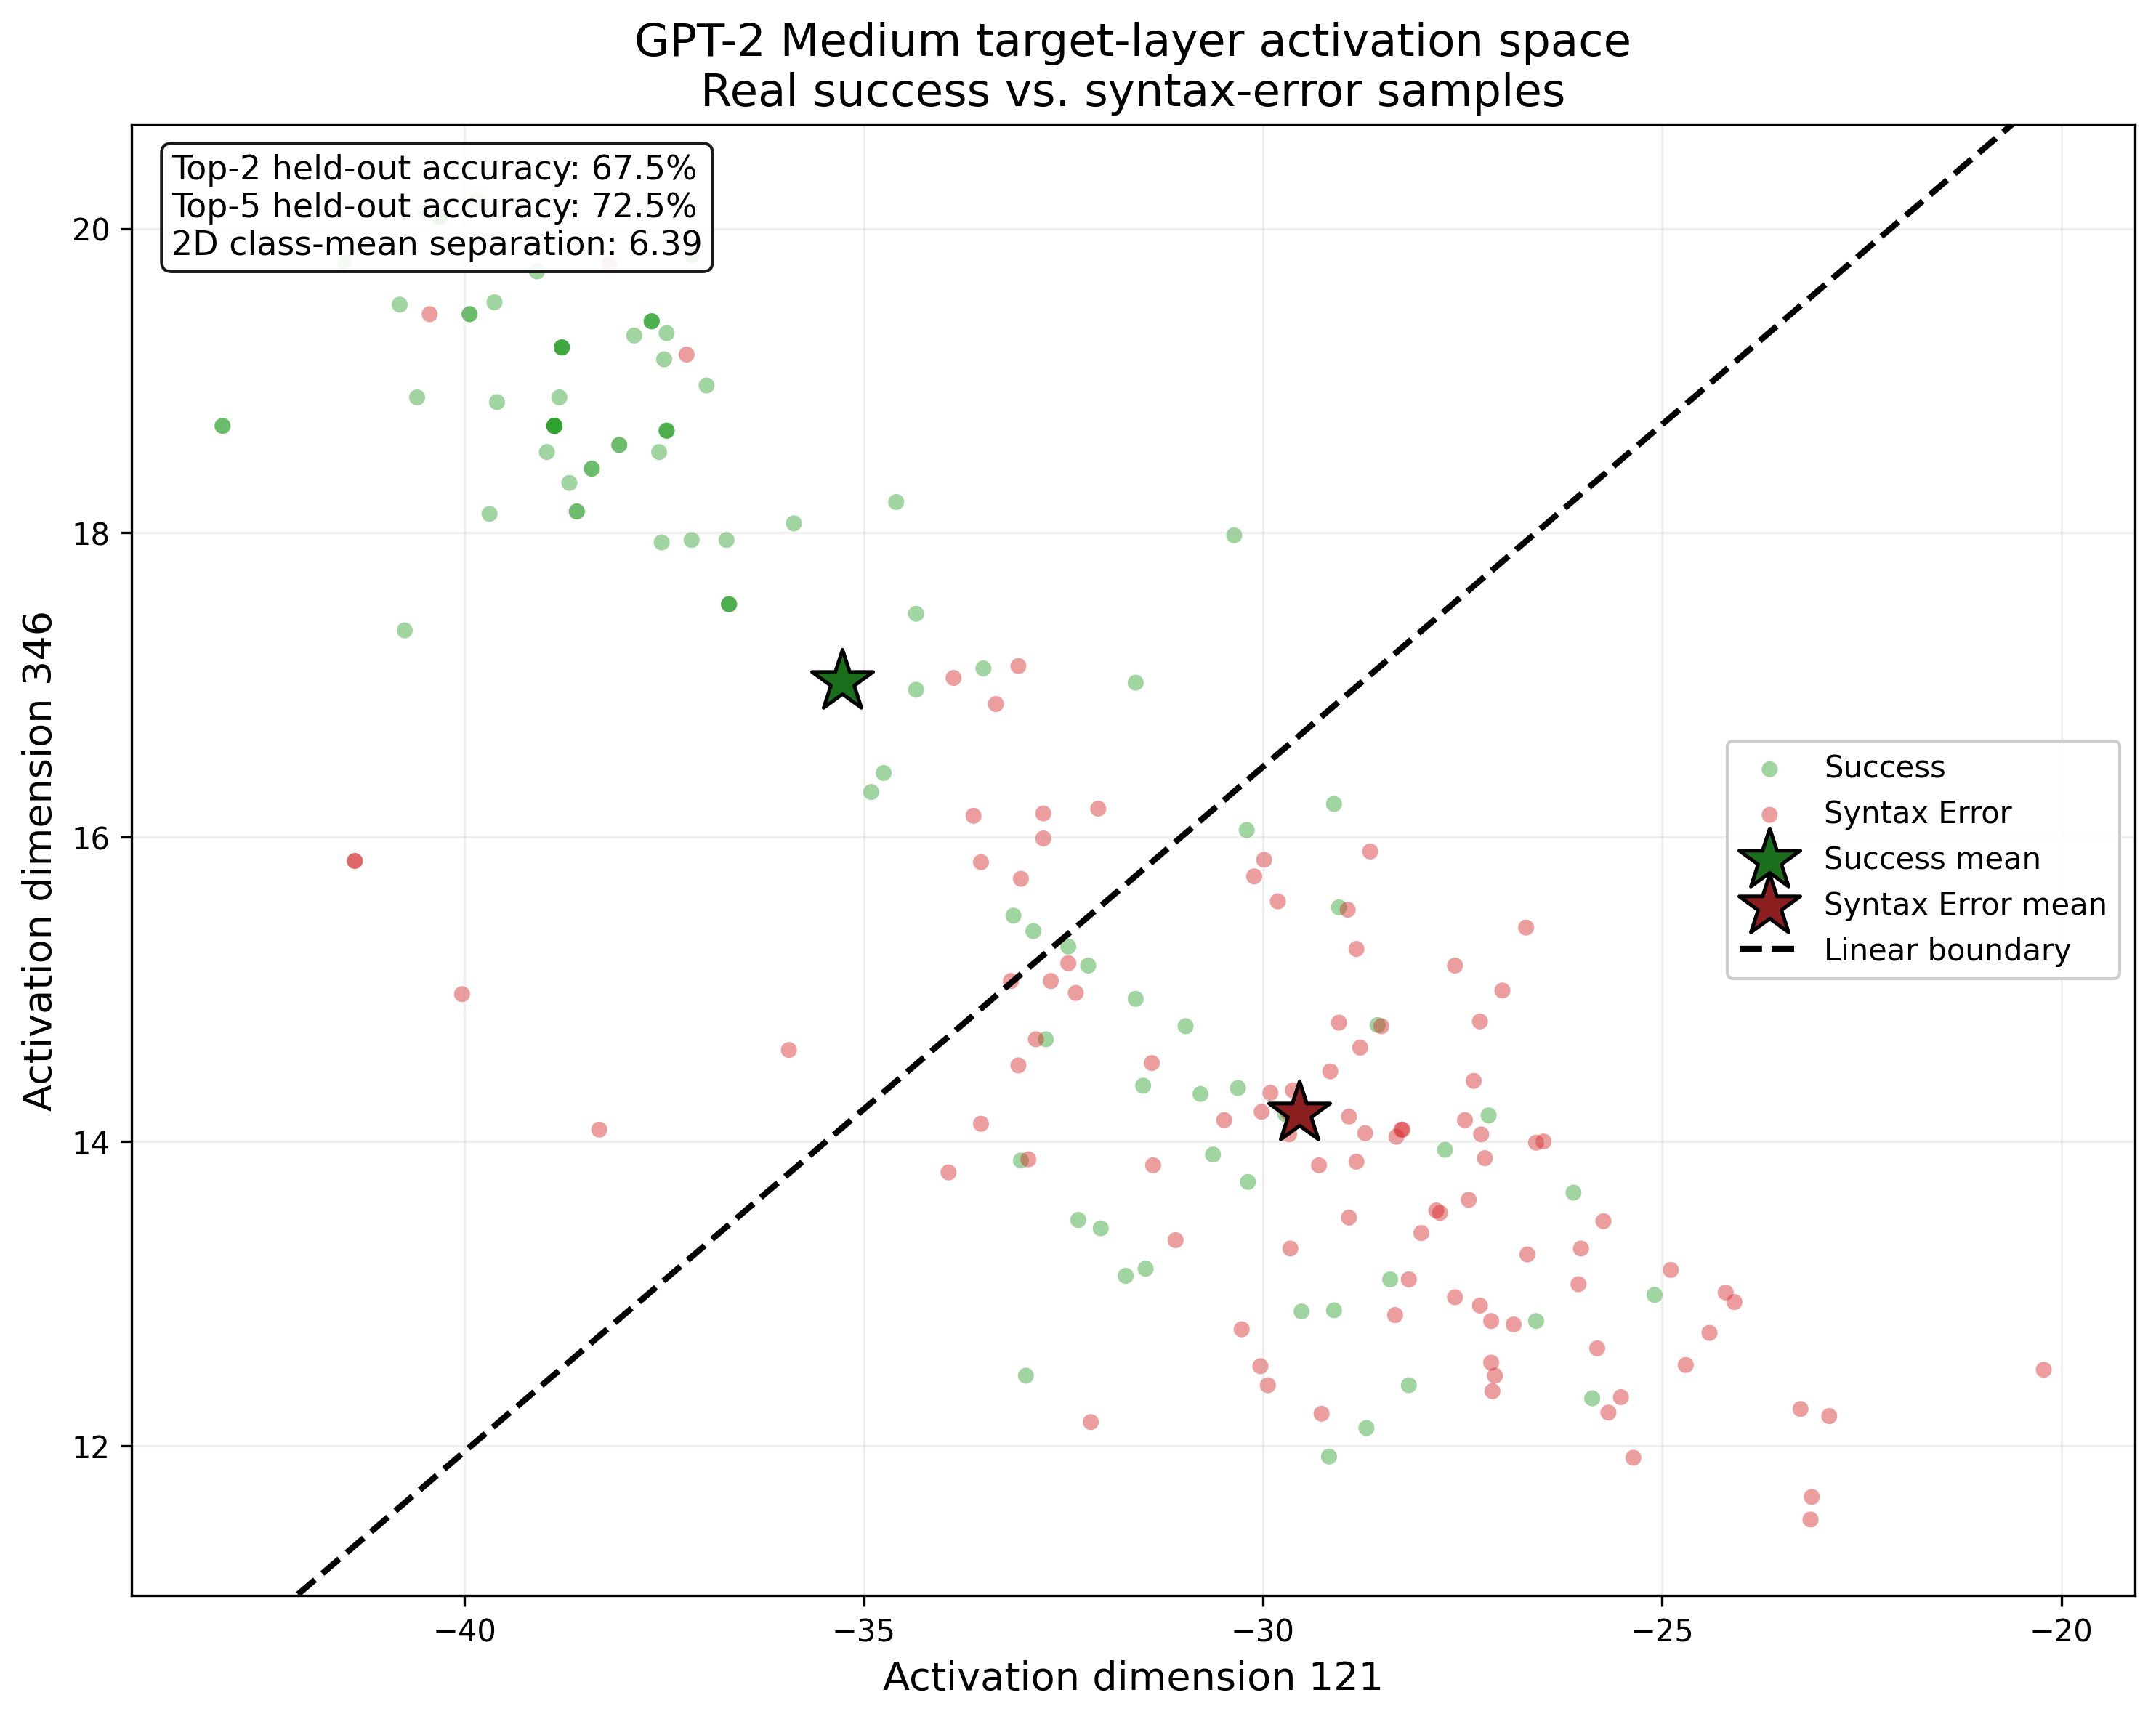
\includegraphics[width=0.9\columnwidth]{figure4_activation_projection_real.png}
\caption{GPT-2 Medium layer-12 activations projected onto the top two discriminative coordinates (121, 346). Success and syntax-failure samples are partially separable, but not cleanly so: the 2D probe reaches 67.5\% accuracy versus 72.5\% for the top-5 probe. The figure should be read as a compact readout, not a full mechanistic decomposition.}
\label{fig:activation_projection}
\end{figure}

\subsection{Cross-Model Comparison: Distinctive Ablation Profiles}
To compare the three models more conservatively, we summarize the most informative ablation signature in each architecture rather than treating a single ``critical depth'' as a universal law.

\begin{table*}[t]
\centering
\caption{Signature Ablation Layers Across Models}
\label{tab:depth_performance}
\footnotesize
\setlength{\tabcolsep}{5pt}
\begin{tabular}{@{}lccc@{}}
\toprule
\textbf{Model} & \textbf{Signature layer} & \textbf{Residual success} & \textbf{Failure mode} \\
\midrule
GPT-2 Small & Layer 2 / 17\% & 1.8\% & 98.2\% syntax \\
GPT-2 Medium & Layer 12 / 50\% & 0.0\% & 76.1\% syntax, 23.9\% runtime \\
CodeGen & Layer 13 / 65\% & 29.5\% & 51.6\% syntax, 18.9\% runtime \\
\bottomrule
\end{tabular}
\end{table*}

\textbf{Finding}: Later signature layers coincide with stronger residual behavior in this three-model comparison, but we treat that pattern as descriptive rather than a scaling law. The clearest contrast is qualitative: GPT-2 Small has only one ablation with any surviving success, GPT-2 Medium has none, and CodeGen retains useful behavior in several layers.

\textbf{Interpretation}: Early signature layers, such as GPT-2 Small's layer 2, suggest that the model commits to correctness before enough context is available. GPT-2 Medium's mid-depth layer 12 instead appears to assemble executable structure without preserving overall fault tolerance. CodeGen's later layer 13 combines the strongest residual success with a mixed syntax/runtime failure pattern, consistent with more distributed code-relevant computation.

\subsection{Scaled Layer-12 Ablation: A Graded Intervention Pilot}

Full zeroing establishes that layer 12 is special, but it does not reveal whether the layer degrades smoothly under weaker interventions. We therefore ran a smaller graded-ablation pilot on GPT-2 Medium layer 12 using 10 HumanEval problems and 5 samples per problem, scaling the layer output by $\{0.75, 0.5, 0.25, 0.0\}$.

\begin{table}[t]
\centering
\caption{Scaled Ablation Pilot for GPT-2 Medium Layer 12}
\label{tab:scaled_layer12}
\footnotesize
\begin{tabular}{@{}lccc@{}}
\toprule
\textbf{Scale} & \textbf{Success \%} & \textbf{Syntax \%} & \textbf{Runtime \%} \\
\midrule
Baseline & 6.0 & 94.0 & 0.0 \\
0.75 & 8.0 & 92.0 & 0.0 \\
0.50 & 2.0 & 98.0 & 0.0 \\
0.25 & 0.0 & 100.0 & 0.0 \\
0.00 & 0.0 & 72.0 & 28.0 \\
\bottomrule
\end{tabular}
\end{table}

\textbf{Finding}: The pilot is too small to treat the 0.75 condition as a stable improvement, but the broader pattern is informative. Partial weakening of layer 12 first drives the model toward near-total syntax collapse, whereas only full removal reproduces the runtime-error regime seen in the main hard-ablation study.

\textbf{Interpretation}: This suggests that layer 12 is not merely a uniformly useful block. Instead, it appears to support a thresholded execution-relevant stage: modest attenuation disrupts syntactic coherence, while complete removal exposes a second regime in which partially executable but incorrect programs survive. That pattern is consistent with layer 12 acting as an assembly point for executable program structure rather than a generic source of accuracy.

\subsection{Constructive Steering and Specificity Controls}

The probe results identify a compact readout, but a stronger mechanistic question is whether the same subspace can be used constructively during generation. We therefore steer GPT-2 Medium layer 12 with the top-5 contrast vector $v=P_5(\mu_{\mathrm{success}}-\mu_{\mathrm{syntax}})$ and compare the result against matched sparse random controls that preserve sparsity and coefficient magnitudes but use different dimensions.

\begin{table}[t]
\centering
\caption{Layer-12 Steering and Matched-Control Pilot}
\label{tab:steering_controls}
\scriptsize
\resizebox{\columnwidth}{!}{%
\begin{tabular}{@{}lccc@{}}
\toprule
\textbf{Condition} & \textbf{Success \%} & \textbf{Syntax \%} & \textbf{Runtime \%} \\
\midrule
Baseline & 6.0 & 94.0 & 0.0 \\
Target $-2.0$ & 10.0 & 90.0 & 0.0 \\
Target $-1.0$ & 2.0 & 94.0 & 4.0 \\
Target $1.0$ & 4.0 & 96.0 & 0.0 \\
Target $2.0$ & 12.0 & 88.0 & 0.0 \\
Random mean ($n=20$) & 6.2 & 92.9 & 0.7 \\
Random max & 14.0 & --- & --- \\
\bottomrule
\end{tabular}
}
\end{table}

\textbf{Finding}: The best learned steering condition ($\alpha=2.0$) doubles subset success from 6.0\% to 12.0\%. Under an expanded set of 20 matched sparse random controls, the control mean remains near baseline at 6.2\%, and the learned vector beats 19 of 20 controls, but one control reaches 14.0\%. We therefore treat the constructive effect as real on this subset while treating the specificity evidence as suggestive rather than conclusive.

\textbf{Interpretation}: The sign pattern is not perfectly monotonic: $\alpha=-2.0$ also improves success to 10.0\%, while $\alpha=-1.0$ introduces a small runtime regime. We therefore interpret the top-5 vector as a \emph{locally useful intervention axis} rather than a globally linear notion of correctness. The strongest supported claim is that the identified subspace is not merely diagnostic, because targeted intervention along it can improve execution. The control comparison still points in the same direction, but with empirical $p \le 0.095$ it does not yet justify a stronger claim of clean subspace specificity.

\begin{figure}[t]
\centering
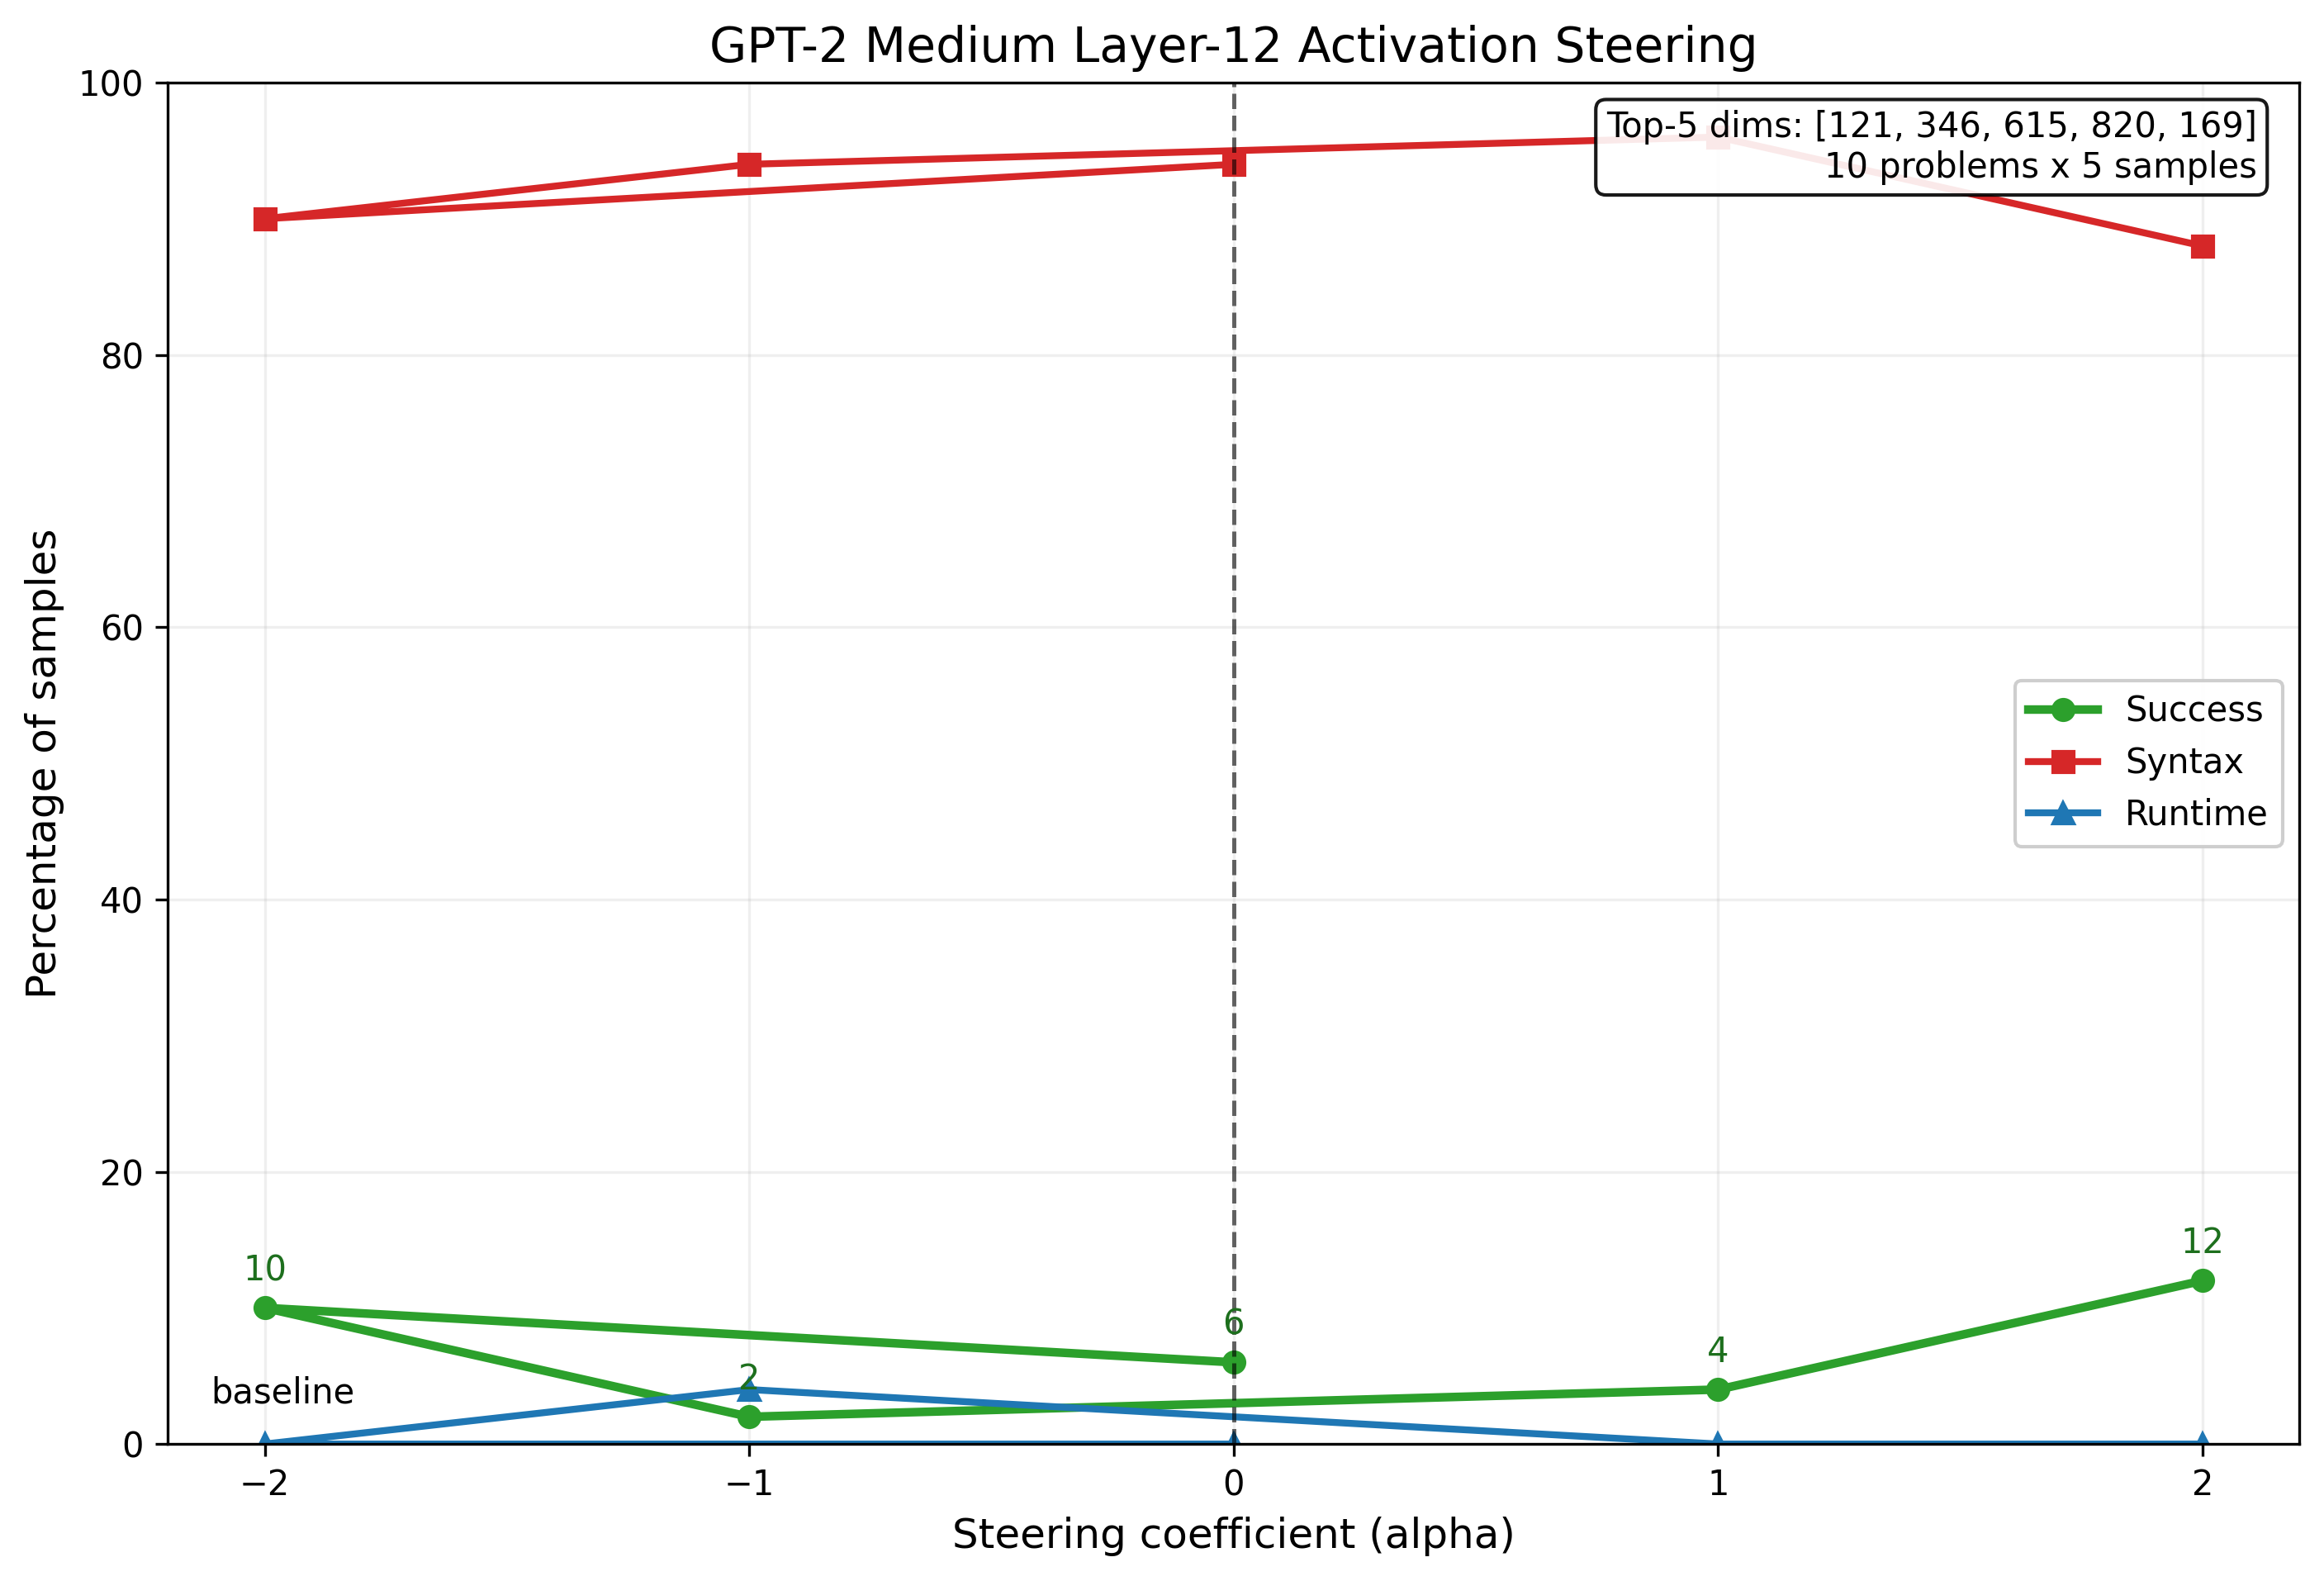
\includegraphics[width=0.9\columnwidth]{figure5_activation_steering_response.png}
\caption{GPT-2 Medium layer-12 steering on the 10-problem / 5-sample subset. The best positive condition doubles success from 6.0\% to 12.0\%, but the response is non-monotonic and strong negative steering also helps. The subspace is therefore intervention-useful without behaving like a single signed correctness axis.}
\label{fig:steering_response}
\end{figure}

\begin{figure*}[t]
\centering
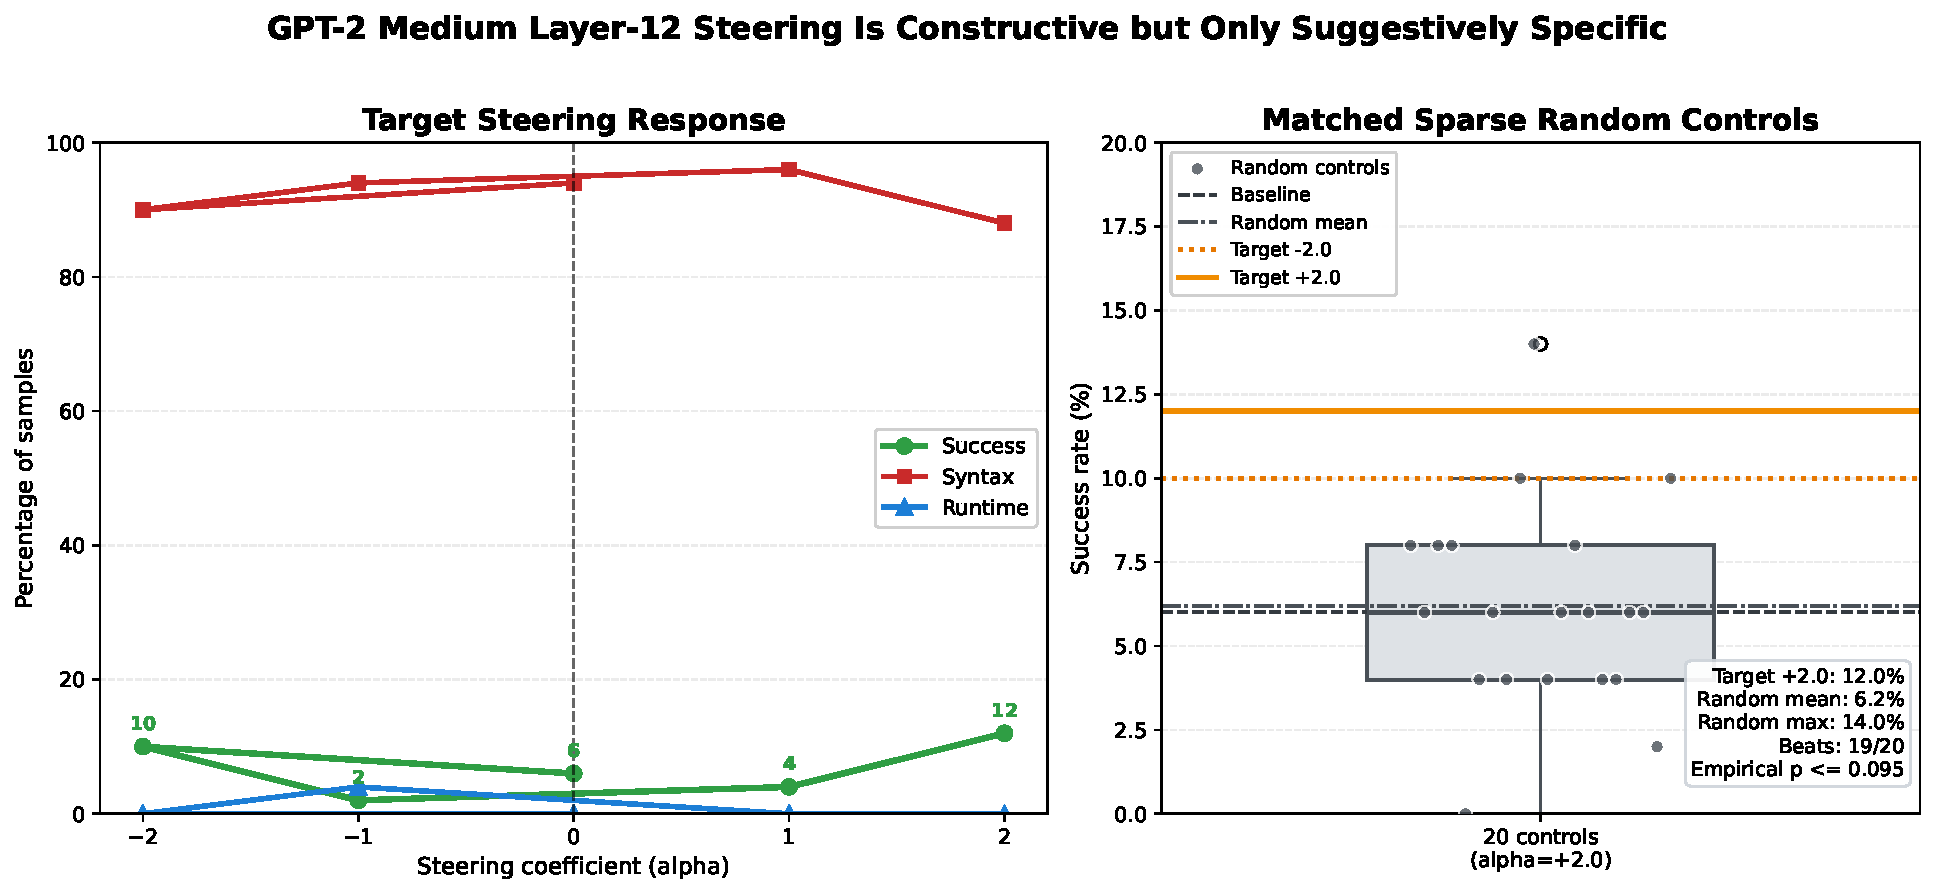
\includegraphics[width=\textwidth]{figure6_steering_controls.pdf}
\caption{Learned steering versus matched sparse controls. The learned vector beats the control mean and 19 of 20 controls, but one random control still reaches 14.0\% success. This supports a useful local intervention more than a clean specificity claim.}
\label{fig:steering_controls_distribution}
\end{figure*}

\subsection{Scaled Layer-13 Ablation in CodeGen}

To test whether the more robust code-specialized model also shows a graded signature, we ran the same 10-problem / 5-sample attenuation study on CodeGen's strongest residual layer (layer 13).

\begin{table}[t]
\centering
\caption{Scaled Ablation Pilot for CodeGen Layer 13}
\label{tab:scaled_layer13_codegen}
\footnotesize
\begin{tabular}{@{}lccc@{}}
\toprule
\textbf{Scale} & \textbf{Success \%} & \textbf{Syntax \%} & \textbf{Runtime \%} \\
\midrule
Baseline & 40.0 & 60.0 & 0.0 \\
0.75 & 28.0 & 72.0 & 0.0 \\
0.50 & 30.0 & 70.0 & 0.0 \\
0.25 & 2.0 & 98.0 & 0.0 \\
0.00 & 24.0 & 52.0 & 24.0 \\
\bottomrule
\end{tabular}
\end{table}

\textbf{Finding}: Unlike GPT-2 Medium, CodeGen does not collapse immediately under partial attenuation. Layer 13 retains 28-30\% success at scales 0.75 and 0.5, collapses to 2.0\% success only at scale 0.25, and still preserves 24.0\% success under full zeroing while shifting 24.0\% of completions into runtime errors.

\textbf{Interpretation}: This is the clearest graded cross-model contrast. GPT-2 Medium layer 12 acts like a brittle thresholded checkpoint, whereas CodeGen layer 13 behaves like a partially redundant execution stage. Even when layer 13 is fully removed, surrounding layers still support a meaningful fraction of executable completions. That is stronger evidence for distributed code-relevant computation than the full-zero ablation table alone.

\begin{figure*}[t]
\centering
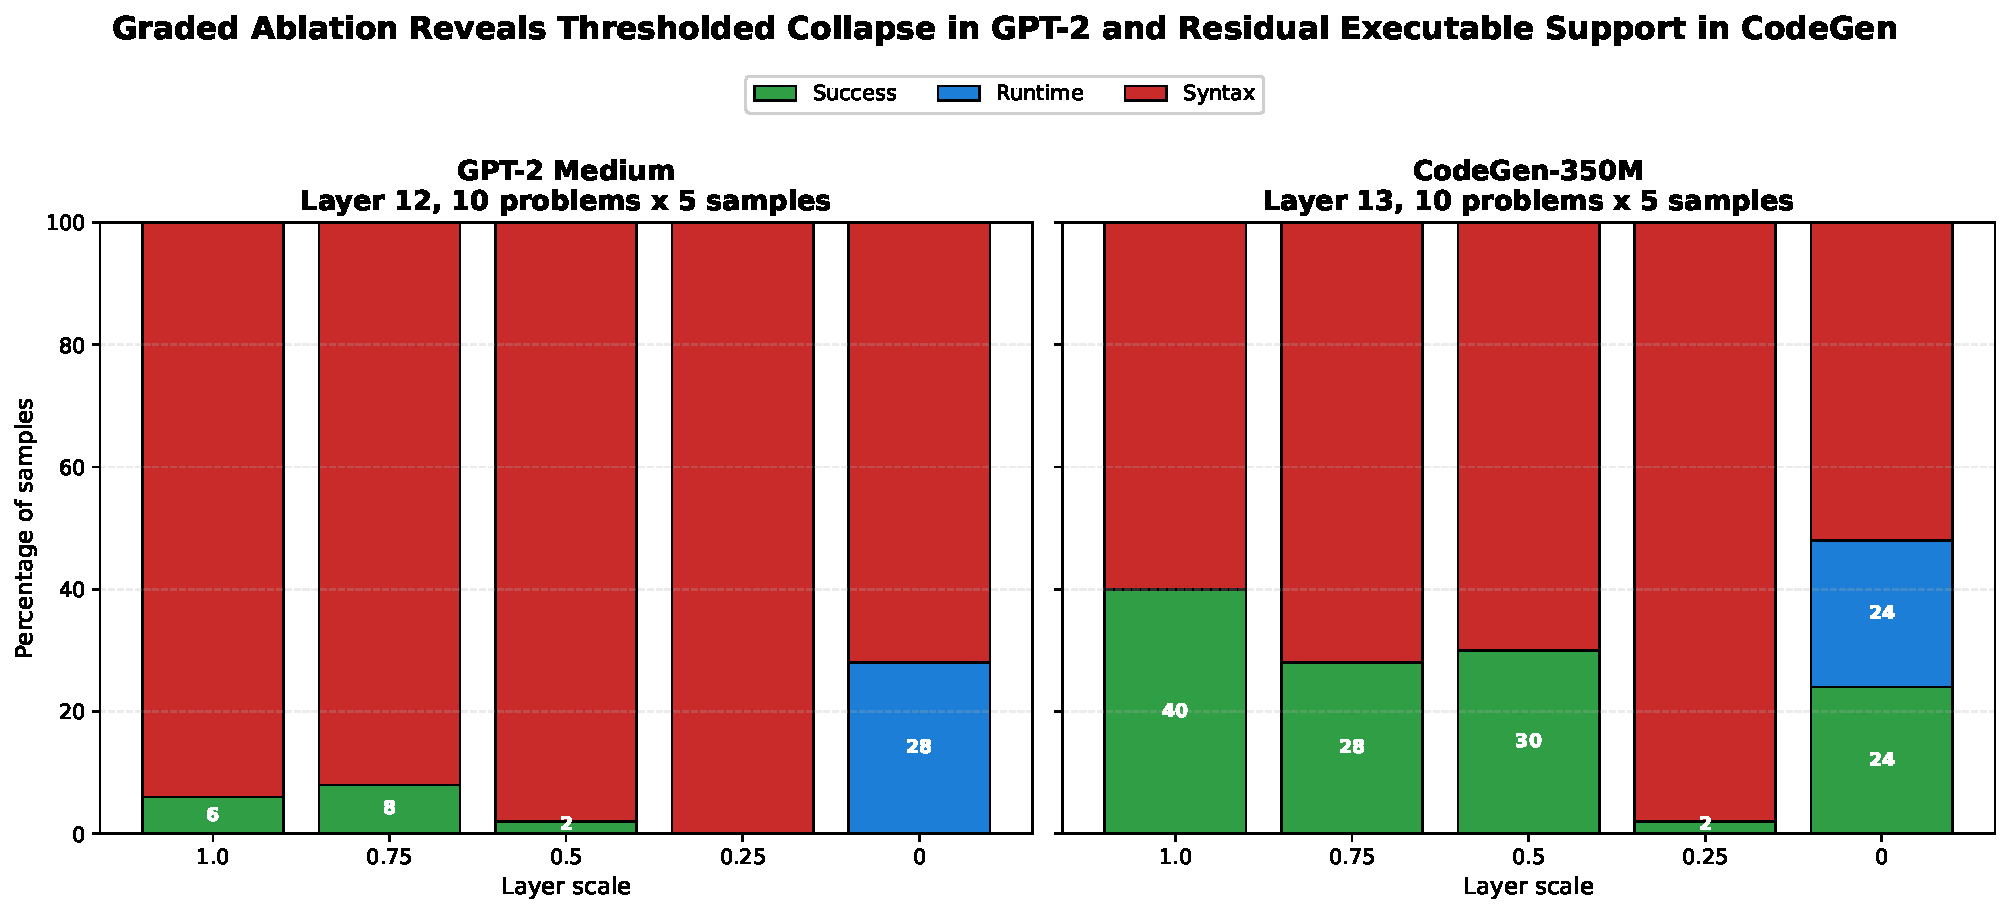
\includegraphics[width=\textwidth]{figure7_scaled_ablation_comparison.pdf}
\caption{Matched graded-ablation comparison of GPT-2 Medium layer 12 and CodeGen layer 13. GPT-2 Medium behaves like a thresholded bottleneck: moderate attenuation drives syntax collapse and only full removal reopens runtime errors. CodeGen retains substantial success under partial attenuation and a mixed success/runtime regime even at zero, consistent with more distributed executable-code support.}
\label{fig:scaled_ablation_comparison}
\end{figure*}
\clearpage
\section{Analysis and Discussion}

\subsection{Why Does Scaling Fail for GPT-2?}

Our ablation results argue against a simple ``larger GPT-2 should inherit more of the same computation'' picture. GPT-2 Medium does not gain broader fault tolerance from added depth: every single-layer ablation drives success to 0\%. Relative to GPT-2 Small, scaling from 12 to 24 layers adds capacity without adding distributed robustness, since Small still retains 1.8\% success at one early layer while Medium retains none anywhere.

What changes is not residual success but the presence of a narrow execution-relevant checkpoint at layer 12. When that layer is removed, 23.9\% of completions become runtime errors rather than collapsing entirely to syntax errors. No other GPT-2 Medium layer shows that behavior. The most plausible interpretation is that the medium model can assemble partially executable programs, but that computation is not distributed strongly enough across neighboring layers to survive a hard intervention.

The graded pilot sharpens the claim. Attenuating layer 12 to 0.5 or 0.25 drives the model toward near-pure syntax collapse, while only full removal reopens a 28.0\% runtime-error regime. We therefore interpret layer 12 as a thresholded assembly stage for executable program structure rather than a redundant contributor that degrades smoothly.

\subsection{How Does CodeGen Achieve Robustness?}

CodeGen's advantage is not that ablations stop mattering. Many single-layer zeroings still reduce success to 0\%, so the intervention remains severe. The difference is structural: useful behavior survives in several layers rather than at one narrow checkpoint. Layers 5 and 7 retain nonzero success, suggesting that early syntactic support is partially distributed, and layer 13 combines the largest residual success (29.5\%) with 18.9\% runtime errors, marking a later executable-code regime.

The graded layer-13 pilot makes the cross-model contrast concrete. At scales 0.75 and 0.5, CodeGen still retains 28--30\% success; only strong attenuation at 0.25 collapses nearly everything into syntax errors, and full zeroing reopens a mixed 24.0\% success / 24.0\% runtime regime. The most economical interpretation is \emph{partial} redundancy: code-relevant computation is spread across neighboring layers even though the model remains vulnerable to severe interventions.

\subsection{What the CodeGen Ladder Adds}

The within-family CodeGen ladder removes the strongest family-difference objection. GPT-2 versus CodeGen alone leaves open tokenization, optimizer, and implementation confounds; NL$\rightarrow$Multi$\rightarrow$Mono keeps architecture and parameter count fixed while changing continued-pretraining data and curriculum.

The ladder still does \emph{not} support an overclean law. HumanEval is not monotone because Multi is slightly worse than NL, so we do not claim a matched-compute or data-only rule. The supported claim is narrower and stronger: within a fixed 350M architecture, later code- and Python-focused continued pretraining materially improves the best checkpoint, and MBPP shows a fully monotone NL$<$Multi$<$Mono progression.

The scaled follow-up strengthens that interpretation without pretending the whole ladder is mechanistically tidy. NL layer 11 behaves like brittle syntax support, Mono layer 13 reopens the mixed runtime regime seen in the main CodeGen model, and Multi remains anomalous under full zeroing. The safest conclusion is therefore that continued pretraining changes both benchmark performance and the geometry of residual code support, even if it does not induce a simple monotone law at every intermediate checkpoint.

\subsection{Implications for Model Design}

Our findings suggest three architectural principles for robust code generation:

\textbf{1. Distribute processing across depth}: Robust models should preserve some residual success or at least diverse failure signatures under harsh interventions, rather than collapsing uniformly at every layer.

\textbf{2. Track failure-mode transitions, not just success collapse}: Layer 12 in GPT-2 Medium is informative precisely because it changes the balance of syntax vs. runtime errors. The new scaled-ablation pilot suggests that this transition is thresholded: syntax collapses first, and the runtime regime appears only after complete removal.

\textbf{3. Code-specific continued pretraining matters}: The GPT-2 checkpoints trained on WebText do not show the same residual robustness profile as CodeGen under our interventions. Code-specific pretraining (The Pile + GitHub)~\cite{gao2021pile,nijkamp2022codegen} is consistent with broader residual robustness under the same intervention, and the within-family CodeGen ladder shows that later code- and Python-focused continued-pretraining stages can improve behavior even without changing architecture or parameter count.

\subsection{Implications for Evaluation Practice}

The targeted robustness controls add a practical lesson for empirical studies of code models: benchmark scores are partly properties of the surrounding generation protocol, not only of the checkpoint. In our saved-artifact controls, prompt format substantially changes HumanEval sample success for the code-specialized models, and MBPP low-temperature decoding increases repeated successful samples while reducing the number of distinct tasks solved at least once.

For software-engineering evaluations, this argues for reporting more than a single aggregate pass rate whenever the goal is reliability. Prompt form, strict-test sensitivity, and task-level coverage should be documented alongside sample-level success so that an apparent gain is not mistaken for broader problem coverage or stronger executable correctness.

\subsection{What the LiveCodeBench Result Changes}

LiveCodeBench sharpens the scope of our claim more than the ranking itself. On HumanEval and MBPP, CodeGen's advantage over GPT-2 is large and practically meaningful. On LiveCodeBench release\_v2, all three small models are near-zero, with CodeGen retaining only a marginal nonzero signal. The right framing is therefore not that small code-pretrained models are broadly strong programmers, but that code-specific pretraining improves classical Python synthesis performance and internal robustness without closing the gap to harder modern coding tasks.

This harsher benchmark is still scientifically useful. It reinforces the negative result because GPT-2 Small and GPT-2 Medium remain indistinguishable at zero, while also preventing us from overclaiming from HumanEval or MBPP alone.

\subsection{Why a Small Probe Still Works}

The five-dimensional probe works because it captures most of the linear separability available in this layer: 72.5\% held-out accuracy versus 75.0\% for the full 1024-dimensional probe. In that operational sense, a very small coordinate set is enough for a strong readout of success versus syntax failure.

That does \emph{not} mean that five neurons implement correctness. The top five dimensions account for only 2.51\% of the total absolute mean shift, so the broader representation remains distributed.

The steering results sharpen the interpretation. The best positive condition doubles success, but one random control still does better and the response curve is non-monotonic. We therefore treat the top-5 subspace as a useful local handle on execution behavior rather than a complete mechanistic decomposition or a signed ``correctness-neuron'' explanation. These dimensions remain promising targets for monitoring and future interventions~\cite{meng2022locating}, but not a complete description of the underlying algorithm.

\subsection{Threats to Validity}

\textbf{Construct validity}: We evaluate executable correctness with benchmark tests. This is appropriate for studying code-generation reliability, but it does not measure maintainability, readability, security, or integration quality. We therefore frame the results as short-form Python synthesis and execution robustness, not as a complete theory of software engineering ability.

\textbf{Internal validity}: The main comparisons depend on fixed decoding settings, saved artifacts, and executor behavior. We reduce this risk by reporting exact sample counts, using problem-level bootstrap tests, separating sample-level and task-level conclusions, and recording the \texttt{HumanEval/129} coverage caveat for the synced CodeGen artifact. The smaller intervention pilots are explicitly treated as causal probes rather than full-benchmark replacements.

\textbf{External validity}: The study covers small decoder-only models, mostly Python tasks, and pretrained checkpoints. The conclusions should not be read as claims about frontier code models, instruction-tuned assistants, repository-level repair, or production deployment. The CodeGen ladder provides a stronger within-family control, but it is still not a matched-compute causal isolation of pretraining data.

\textbf{Conclusion validity}: Several results are intentionally framed conservatively. The GPT-2 Small versus Medium HumanEval gap is numerically small and not statistically reliable. The steering result improves subset success, but one matched random control outperforms the learned vector, so we claim a locally useful intervention axis rather than a definitive sparse mechanism. This conservative framing is part of the evidentiary standard rather than a rhetorical limitation.

\subsection{Limitations and Future Work}

The validity threats above imply several direct extensions:

\textbf{1. Benchmark scope is broader but still limited}: We evaluate on HumanEval, HumanEval+, MBPP, MBPP+, and contamination-aware LiveCodeBench~\cite{chen2021humaneval,austin2021program,liu2023evalplus,jain2024livecodebench}, which is stronger than the earlier two-benchmark version, but all settings still emphasize short-form code-generation tasks rather than long-horizon repository-level software engineering.

\textbf{2. Pretrained models only}: We do not evaluate fine-tuned models. While our goal was to isolate base architecture effects, fine-tuning could potentially repair GPT-2 Medium's bottleneck by redistributing computation across layers.

\textbf{3. The CodeGen ladder is controlled but not matched-compute}: NL, Multi, and Mono hold architecture and parameter count fixed, but they also differ in additional tokens, optimization steps, and curriculum. The ladder therefore supports a strong within-family continued-pretraining claim, not a perfectly factorized causal isolation of data distribution alone.

\textbf{4. Graded interventions remain limited}: We include scaled-ablation pilots for GPT-2 Medium layer 12, CodeGen layer 13, and a final ladder follow-up on CodeGen-NL / Multi / Mono signature layers. Even so, these remain small targeted subsets rather than full benchmark sweeps, and one ladder leg (CodeGen-Multi layer 7) behaved anomalously under full zeroing. Broader graded sweeps remain necessary before claiming a general law of thresholded behavior.

\textbf{5. Limited semantic analysis}: We identify which layers validate syntax but do not deeply analyze which layers perform semantic reasoning (variable scoping, type consistency, algorithm correctness). Future work should extend our methods to semantic error detection.

\textbf{6. Constructive intervention evidence is still small-scale}: We observe positive rescue from learned steering on a subset, and the learned vector beats 19 of 20 matched sparse random controls, but one control does better and the empirical control test remains only suggestive ($p \le 0.095$). Larger control sets and cross-benchmark steering experiments are needed before treating the subspace as a robust causal handle.

Despite these limitations, our core finding is that code models differ not only in accuracy but in their layerwise failure profiles under intervention, providing actionable insight for model design and evaluation.

\subsection{Reproducibility and Artifact Availability}

This paper is intended to be artifact-traceable rather than narrative-only. The quantitative claims in the main text are backed by saved processed outputs under \texttt{outputs/tables/}, benchmark result files under \texttt{data/results\_*/}, figure-generation scripts under \texttt{scripts/}, and the claim-to-artifact audit included with the review package. In particular, the benchmark-summary figures are regenerated from saved bootstrap summaries, strict-evaluation summaries, LiveCodeBench summaries, and repaired CodeGen ladder artifacts rather than from hand-copied spreadsheet values.

The intended submission package includes a supplementary archive containing the processed tables, benchmark result artifacts, analysis scripts, source code, configuration files, plotting scripts, figures, and audit reports needed to trace the reported numbers. Raw local execution logs are preserved in the working repository but are not required for the reviewer-facing package because the reported claims are checked against the structured summaries and artifacts. A public archival repository can be created from this curated archive after the review-facing version is accepted or explicitly requested. We keep the main-paper coverage note for \texttt{HumanEval/129} explicit because reproducibility includes honest accounting of what was and was not saved in the synced main CodeGen artifact.

\subsection{Broader Impact}

The immediate positive impact of this work is methodological. Better tools for diagnosing where code models fail can improve evaluation practice, reduce overclaiming from small benchmark gains, and help future systems distribute executable-code behavior more robustly across depth. The strongest practical message is not that small models are already good programmers, but that pretraining choices and failure-mode analysis deserve at least as much attention as raw scale in this regime.

The main risk is dual use. Mechanistic insight into code-generation bottlenecks, especially if paired with constructive steering or future stronger interventions, could eventually be used to make automated code generation more capable for both beneficial and harmful ends, including insecure code production or malicious automation. We partially mitigate that risk by studying small openly available models, by emphasizing reliability analysis over deployment recipes, and by treating the steering results as limited scientific evidence rather than as a production-ready capability-improvement method.

\section{Conclusion}

We show that, in this small-model regime, the conventional expectation that ``bigger models are better'' does not hold reliably for code generation: GPT-2 Medium (355M parameters) fails to improve meaningfully over GPT-2 Small (124M parameters) despite 2.9$\times$ more parameters.

Problem-level bootstrap analysis makes this conclusion more precise: GPT-2 Small and GPT-2 Medium are statistically indistinguishable on HumanEval in our setting, whereas both remain more than 30 percentage points behind CodeGen-350M with highly significant pairwise differences.

The same claim transfers to full-coverage MBPP. Across 257 tasks with 20 samples each, GPT-2 Small and GPT-2 Medium both achieve 0.0\% success, whereas CodeGen-350M reaches 7.39\% success and 22.96\% pass@5. The pairwise MBPP success-rate gaps against CodeGen remain highly significant ($p=0.0001$), while the GPT-2 Small vs. GPT-2 Medium difference vanishes entirely ($p=1.0$).

A stricter HumanEval+ re-evaluation preserves the same ordering. On the first five saved samples per task, GPT-2 Small and GPT-2 Medium both remain at 0.0\% pass@1, whereas CodeGen-350M retains 2.1\% pass@1 after the augmented hidden tests.

The same conclusion survives a separate strict MBPP+ evaluation with EvalPlus. On 378 tasks scored under the stronger Base+Extra metric, GPT-2 Small and GPT-2 Medium both remain at 0.0\% pass@1 and pass@10, whereas CodeGen-350M retains 1.1\% pass@1 and 6.4\% pass@10.

The contamination-aware LiveCodeBench result narrows and strengthens the paper at the same time. GPT-2 Small and GPT-2 Medium remain at 0.0\% on pass@1, pass@5, and pass@10, while CodeGen-350M remains only marginally above zero (0.02\%, 0.10\%, and 0.20\%). Thus, the strongest positive comparative result remains concentrated on HumanEval and MBPP, but the negative conclusion that scale alone is insufficient survives even under a much harder modern benchmark.

The within-family CodeGen ladder sharpens the paper further. At fixed 350M scale, CodeGen-Mono is strongest on both HumanEval and MBPP, while the MBPP ladder is cleanly monotone from NL to Multi to Mono and the HumanEval ladder is full-coverage but mixed at the intermediate Multi checkpoint. Because the checkpoints receive additional compute and curriculum, we interpret this not as a pure data-only law but as strong within-family evidence that later code- and Python-focused continued pretraining materially improves small-model code generation.

Under full-layer ablation, GPT-2 Medium never preserves success; instead, layer 12 stands out because its removal uniquely shifts 23.9\% of failures into runtime errors while every other layer collapses almost entirely to syntax errors.

A graded layer-12 pilot strengthens this interpretation. Partial attenuation first pushes GPT-2 Medium toward complete syntax collapse, while only full zeroing reopens a 28.0\% runtime-error regime. This suggests that layer 12 marks a thresholded execution-relevant stage rather than a smoothly redundant computation.

In contrast, CodeGen-350M~\cite{nijkamp2022codegen} still shows severe sensitivity to hard ablation, but it exhibits broader residual robustness than either GPT-2 variant. Four layers retain nonzero success, and the graded layer-13 pilot preserves 28-30\% success under partial attenuation and 24.0\% success even under full zeroing, indicating that code-relevant computation is less concentrated than in GPT-2. The final ladder follow-up is consistent with that picture at the two clean checkpoints: CodeGen-NL layer 11 degrades toward syntax collapse under attenuation, whereas CodeGen-Mono layer 13 again preserves a mixed executable/runtime regime under full zeroing.

Our activation analysis shows that a compact probe on five layer-12 dimensions (121, 346, 615, 820, 169) reaches 72.5\% held-out accuracy, close to the 75.0\% achieved by a full-layer linear probe. More importantly, constructive steering along this same sparse direction doubles subset success from 6.0\% to 12.0\%. The expanded random-control comparison is favorable but not decisive, so the safest conclusion is that this direction is a usable local control subspace rather than a purely descriptive probe.

The targeted robustness controls add a systems-level caution to that mechanistic claim. Prompt format and decoding temperature can substantially change sample-level success, and on MBPP low-temperature decoding improves repeated sample success while reducing distinct-task coverage. Thus, the bottleneck is partly internal to the model and partly induced by the generation/evaluation protocol around it.

These findings challenge the scaling-centric paradigm in neural code generation~\cite{kaplan2020scaling,wei2022emergent}. Parameter count alone does not determine capability. Across HumanEval, HumanEval+, MBPP, MBPP+, and a harsher contamination-aware LiveCodeBench stress test, the central predictor of useful code behavior in this small-model regime is not scale within the GPT-2 family, but whether pretraining has already distributed code-relevant computation across depth. The within-family CodeGen ladder makes this point harder to dismiss: even with architecture and parameter count held fixed, later continued-pretraining stages can materially change both performance and the layerwise organization of executable-code behavior. For practitioners, the main design lessons are to distribute code-relevant processing across depth, analyze failure-mode shifts under intervention, and use code-specific pretraining to build residual robustness.

Future work should extend our mechanistic analysis to fine-tuned models, multilingual code generation, and semantic error detection, with the ultimate goal of reverse-engineering the complete algorithms by which neural networks generate syntactically and semantically correct programs.

\section*{Data Availability}

The processed result tables, plotting scripts, benchmark summaries, saved result artifacts, configuration files, source code, and claim-to-artifact audit used in this manuscript are available in the \submissionartifact{} submitted with this manuscript. Large model checkpoints and raw model caches are not redistributed; all experiments use public pretrained checkpoints and regenerate derived outputs from the provided scripts and configuration files.

\section*{Declaration of Competing Interest}

The author declares no known competing financial interests or personal relationships that could have appeared to influence the work reported in this paper.

\section*{Funding}

This research did not receive any specific grant from funding agencies in the public, commercial, or not-for-profit sectors.

\section*{Declaration of Generative AI and AI-Assisted Technologies in the Manuscript Preparation Process}

During the preparation of this work, the author used OpenAI Codex to assist with manuscript editing, code execution orchestration, artifact organization, and formatting. After using this tool, the author reviewed and edited the content as needed and takes full responsibility for the content of the submitted manuscript.

\appendix

\section{Supplementary Benchmark and Provenance Figures}

The main paper emphasizes the benchmark-wide result map, bootstrap intervals, and within-family CodeGen ladder. We place two additional supporting figures here for transparency: a pass@1 strictness cascade across benchmark families and a provenance-oriented coverage audit for the repaired HumanEval artifacts.

\begin{figure*}[t]
\centering
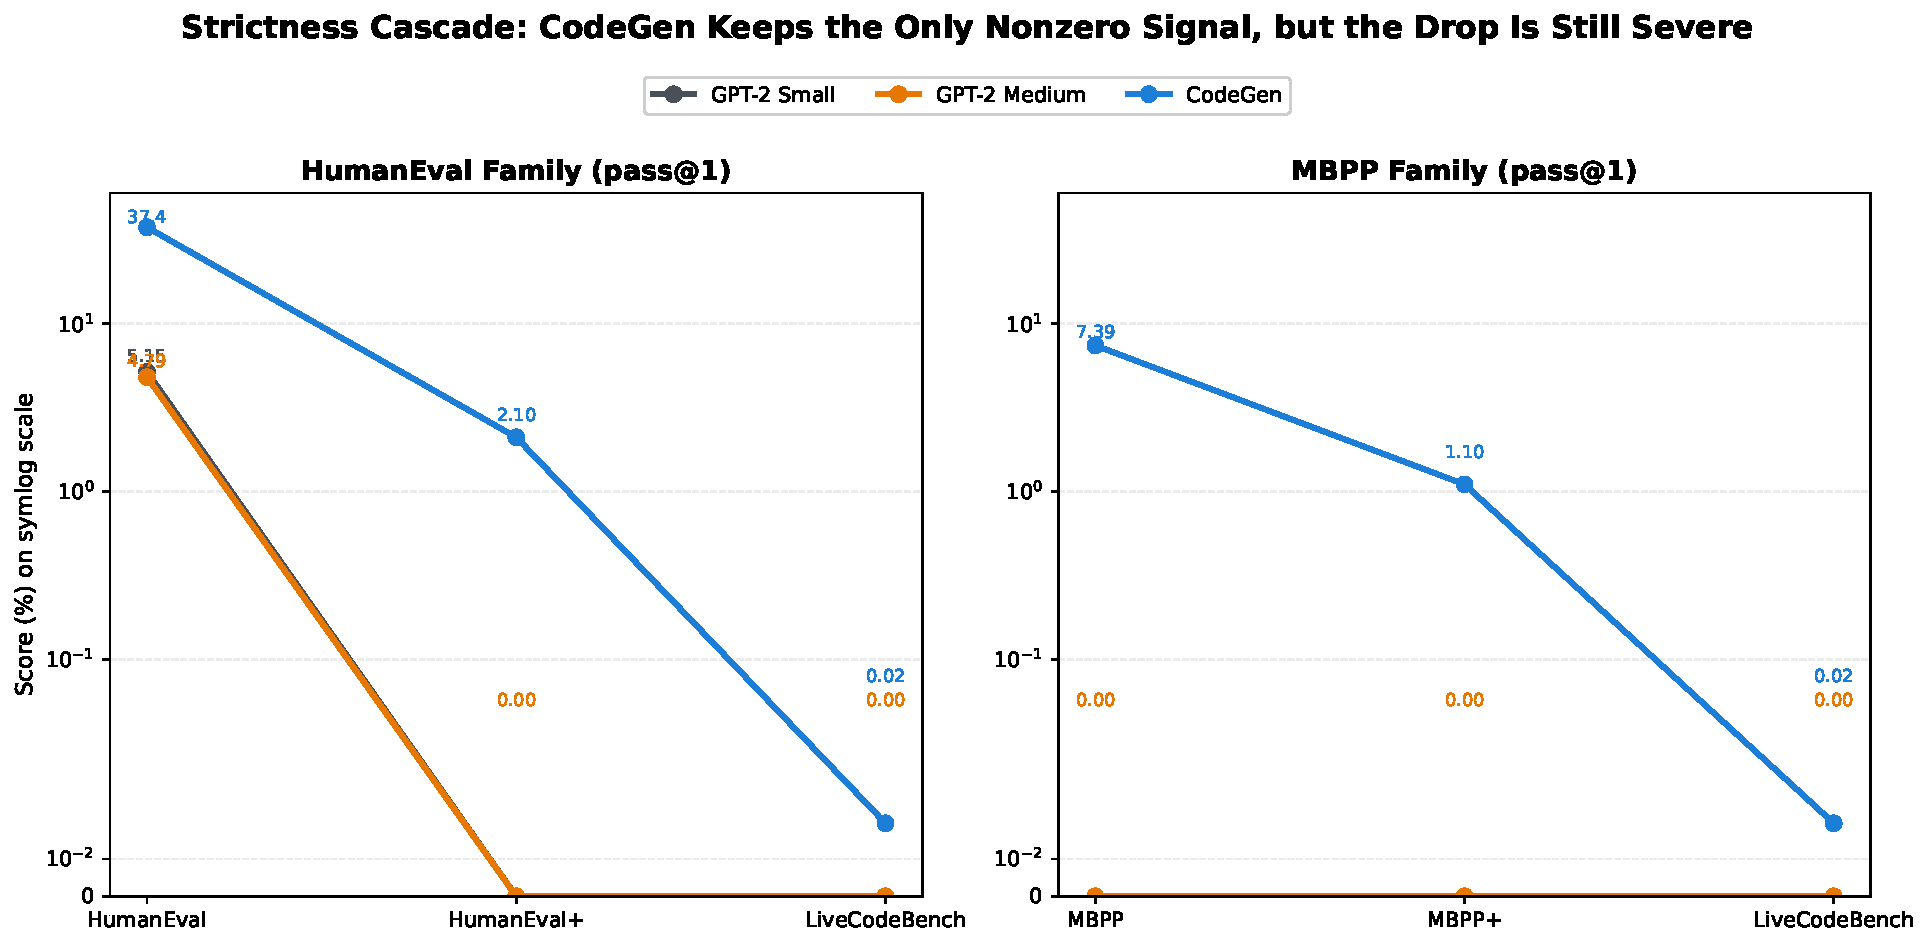
\includegraphics[width=\textwidth]{figure13_strictness_cascade.pdf}
\caption{Pass@1 cascade across benchmark families. CodeGen retains the only nonzero signal as evaluation becomes stricter, but the drop from classical benchmarks to HumanEval+/MBPP+ and LiveCodeBench is severe. GPT-2 Small and GPT-2 Medium remain indistinguishable at or near zero throughout.}
\label{fig:strictness_cascade}
\end{figure*}

\begin{figure*}[t]
\centering
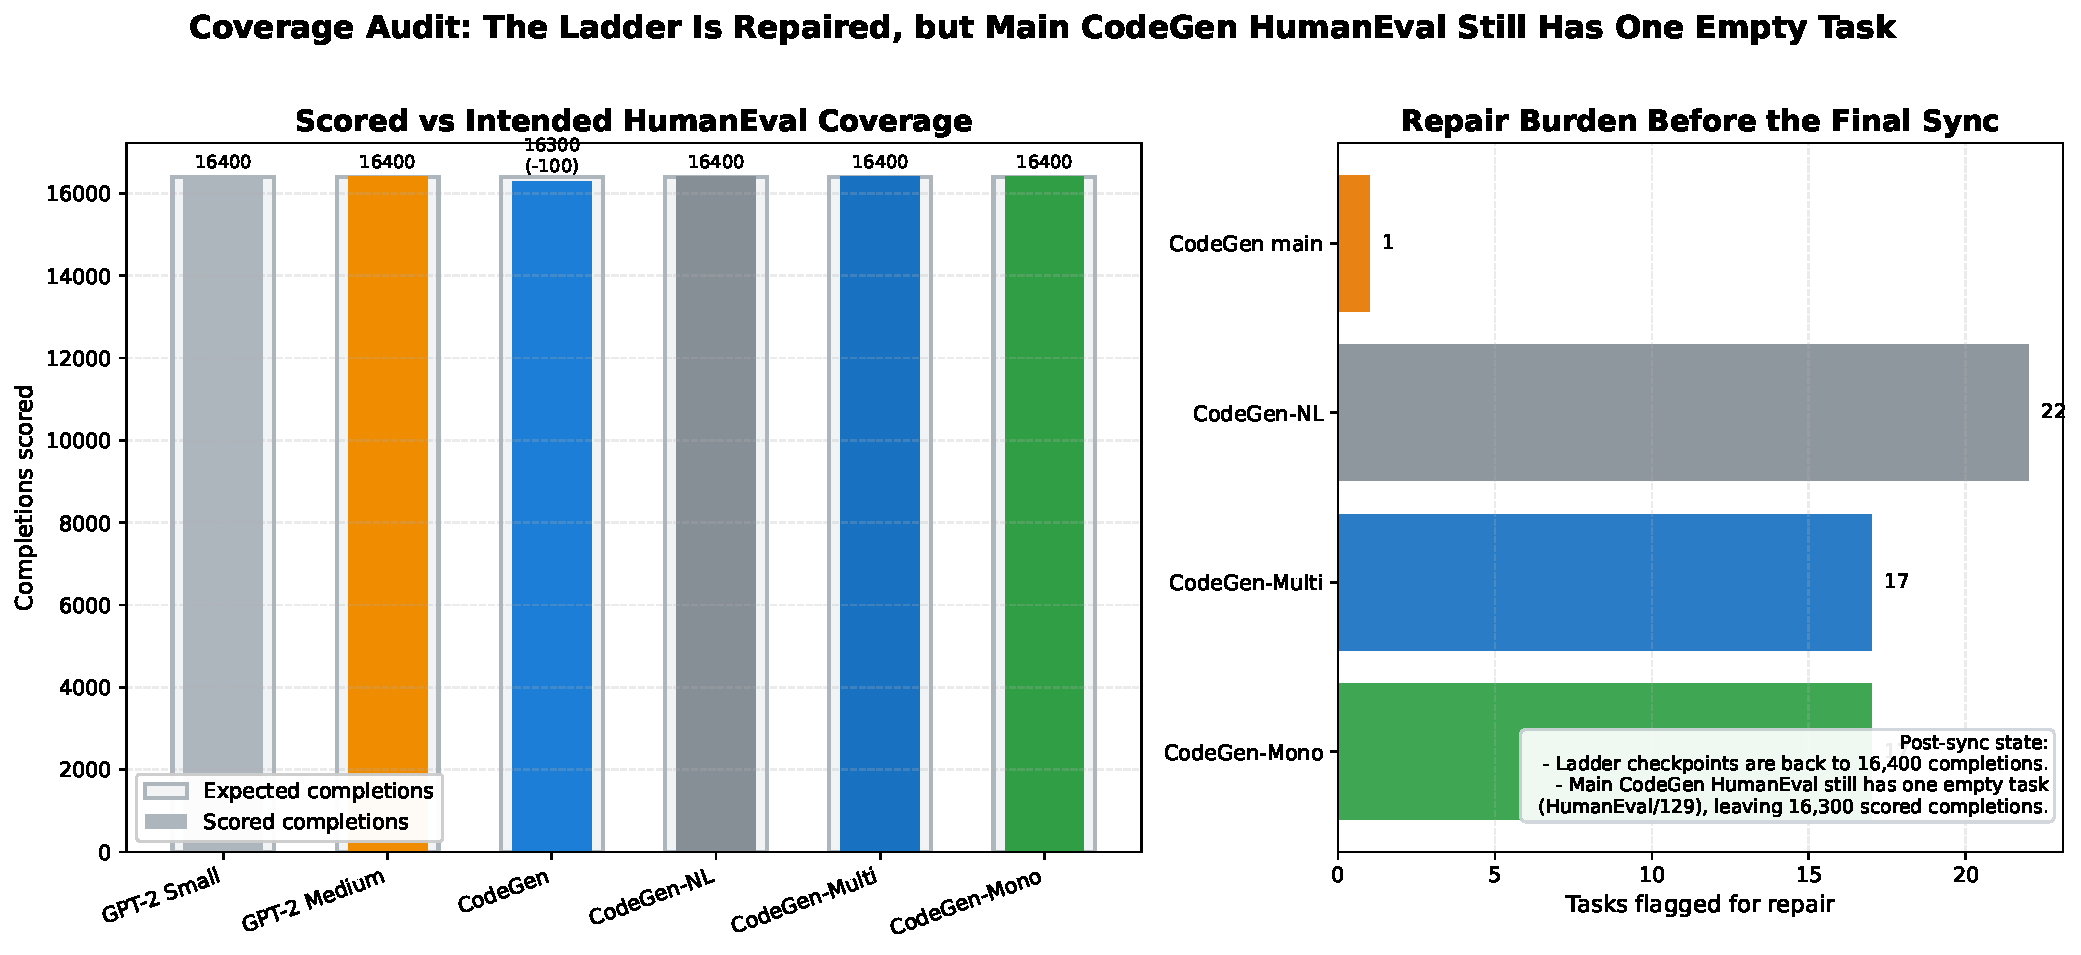
\includegraphics[width=\textwidth]{figure14_coverage_audit.pdf}
\caption{Coverage and repair audit for the final HumanEval artifacts. The repaired CodeGen ladder checkpoints return to full 16,400-completion coverage, while the synced main CodeGen HumanEval artifact still contains one empty task (\texttt{HumanEval/129}), leaving 16,300 scored completions. The right panel records the pre-sync repair burden that produced the final ladder artifacts.}
\label{fig:coverage_audit}
\end{figure*}

\bibliographystyle{elsarticle-harv}
\bibliography{references}

\end{document} 
